\documentclass[header.tex]{subfiles}
\begin{document}
\title{\plaintitle}

\numberofauthors{3}
\author{%
  \alignauthor{Leave Authors Anonymous\\
    \affaddr{for Submission}\\
    \affaddr{City, Country}\\
    \email{e-mail address}}\\
  \alignauthor{Leave Authors Anonymous\\
    \affaddr{for Submission}\\
    \affaddr{City, Country}\\
    \email{e-mail address}}\\
  \alignauthor{Leave Authors Anonymous\\
    \affaddr{for Submission}\\
    \affaddr{City, Country}\\
    \email{e-mail address}}\\
}




\teaser{
%\begin{figure}
\centering
\includegraphics[width=1\textwidth]{figures/Fig1_Nur}
\caption{Sketch\&Stitch walkthrough: (a) A user sketches artwork directly on fabric, (b) she uses \textit{Circuit Stickers} to plan the circuit layout, (c) she draws circuit traces to connect the stickers, (d) the system takes a picture of the sketch, converts it into embroidery patterns, and sends them to an embroidery machine for stitching using conductive and non-conductive threads, (e) the user replaces Circuit Stickers with real electrical components and attaches them to the fabric.
}
 \vspace{-1em}
\label{fig:Fig1}
}

\maketitle



\begin{abstract}
E-Textiles are fabrics that integrate electronic circuits and components. Makers use them to create interactive clothing, furniture, and toys. However, this requires significant manual labor and skills, and using technology-centric design tools. We introduce \textit{Sketch\&Stitch}, an interactive embroidery system to create e-textiles using a traditional crafting approach: Users draw their art and circuit directly on fabric using colored markers. The system takes a picture of the sketch, converts it into embroidery patterns, and sends them to an embroidery machine. Alternating between sketching and stitching, users build and test their design incrementally. Sketch\&Stitch features \textit{Circuit Stickers} representing circuit boards, components, wire crossings to insulate, and various textile touch sensors such as pushbuttons, sliders, and 2D touchpads. Circuit Stickers serve as placeholders during design. Using computer vision, they are recognized and replaced later in the appropriate embroidery phases. We close with technical considerations and application examples.
\end{abstract}


\category{H.5.2}{User Interfaces}{}

\keywords{\plainkeywords}

\section{Introduction}


Electronic textile technology enables people to create expressive, interactive, and functional textile artifacts for both playful and serious applications.
It combines the visual and haptic expressiveness of textiles with the interactivity and utility of electronic components such as LEDs, vibration motors, speakers, GPS receivers, and touch sensors. At the intersection of technology, art, and fashion (see, e.g., CuteCircuit.com), e-textiles have attracted artists, designers, hobbyists, and makers applying this technology in creative and artistic ways \cite{berzowska2005kukkia,Buechley:2010:LWH:1858171.1858206}. 
%Other e-fashion companies:
%https://iq.intel.com/fashion-metamorphosis-meet-the-butterfly-dress/
%http://ezratuba.com/wearable-tech
%Berlin University of the Arts - Department of Textile and Surface Design
This has motivated HCI research to investigate techniques that enable a wider audience to integrate fabrics and electronics into interactive textiles \cite{Buechley2009,perner2011handcrafting,5387040}.

In e-textiles, conductive threads, inks, polymers, or textiles are attached directly to a base fabric, creating \textit{fabric circuits}. These circuits connect traditional electronic components, usually on printed circuit boards, but they can also directly include functional parts such as fabric-based resistors, capacitors, touch sensors, actuators \cite{stylios2007shape}, or antennas \cite{catrysse2004towards}.
%batteries \cite{}
%powering elements \cite{}
Creating e-textiles typically involves 1.\ designing or choosing an artwork, 2.\ planning the layout of electrical components and traces, 3.\ creating the artwork and fabric circuit on the base fabric, 4.\ insulating circuit traces where necessary, and 5.\ attaching electronic components \cite{Lovell:2010:ETD:1810543.1810578}. 
The techniques for implementing e-textiles are based on traditional methods such as weaving \cite{kallmayer2003new}, embroidery \cite{5387040}, and printing \cite{kim2010electrical}.
%\cite{castano2014smart,mattila2006intelligent}. These citations provide a review of methods

%Some of these techniques have been successfully adopted by the do-it-yourself community 
% as evident from makers' websites, such as Instructables\footnote{https://www.instructables.com/}, Sparkfun\footnote{https://www.sparkfun.com/} and Adafruit\footnote{https://www.adafruit.com/}. But these techniques have some constraints.
%More websites: https://www.lib.ncsu.edu/softcircuits


As users rely predominantly on manual implementation of e-textiles \cite{Kazemitabaar:2017:MTA:3025453.3025887}, executing a design becomes labor-intensive and requires high skill levels as the number and density of electrical components and connections increase. Debugging e-textiles is only possible after investing considerable time in building them. Insulating circuit traces is an extra step requiring special tools and materials \cite{Buechley2009}. Observing participants in our e-textile workshops, and analyzing over 70 e-textile projects documented online, we found that this laborious multi-step process often forced them into trade-offs between the visual and functional aspects of their design, impeding improvisation and exploration. The lack of a design pipeline and digital support for e-textile fabrication can thus limit the creative and iterative design of e-textiles.
%enable users to focus and invest their time on the visual and functional aspects of their project.

% We analysed more than 70 e-textile projects on the mentioned websites and found that makers make a trade-off between the fidelity of the artistic pattern and the functionality of the artefact. 


In this paper, we present \textit{Sketch\&Stitch,} an interactive embroidery system that enables users to create e-textiles by sketching on fabric (Fig.~\ref{fig:Fig1}). It uses a computerized embroidery machine as a digital fabrication tool to handle the two most laborious steps when creating e-textiles, stitching and insulation. Sketch\&Stitch features \textit{Circuit Stickers}, printed adhesives representing elements users can embed into their design, from circuit boards and components, to wire crossings to insulate, to various textile touch sensors. These stickers guide the user while drawing circuit traces to ensure reliable electrical connections, and are recognized using computer vision, automatically generating stitching patterns for sensors, insulations, and wire crossings, for example.

% In Sketch\&Stitch, a user begins by sketching an artwork on the workpiece fabric using colored fabric markers. She plans the placement of components using Circuit Stickers and draws connections. When she is ready to execute the design, the system takes a picture of the sketch, converts it into embroidery patterns, and sends them to an embroidery machine. 
% %The embroidery machine's embedded display allows the user to verify the patterns and make minor adjustments before stitching is started. 
% The user may repeat these steps to review and test parts of her art and circuitry incrementally. Some Circuit Stickers, e.g., for touch sensors, are already replaced with stitches automatically by the system. After embroidery is complete, the user replaces the remaining Circuit Stickers with their component counterparts, using one of three attachment techniques we describe.

In the remainder of this paper, after reviewing related work, we first briefly introduce the reader to the particular features of computerized embroidery machines that are relevant for this work. We present Sketch\&Stitch and its interaction design. We illustrate the extensions we added to Sketch\&Stitch beyond the basic system that enable a wider range of practical applications, and walk the reader through a concrete example. After providing details on the software implementation and recommendations for materials and stitching techniques, we present several example artifacts created using our system, and close by discussing the current limitations of Sketch\&Stitch and opportunities for future research.

In summary, this paper makes the following contributions:
\begin{itemize}
    \item Sketch\&Stitch, a new approach and system prototype to create e-textiles by drawing directly on the fabric;
    \item Interaction techniques and embroidery patterns that let users include circuit boards, components, insulation, wire crossings, and a variety of fabric sensors using Circuit Stickers;
    \item Technical recommendations for materials and stitching processes to create e-textiles with digital embroidery machines.
\end{itemize}


% Machine embroidery has bloomed entering homes, makerspaces and design studios of crafters, hobbyists and DIY.

% \url{http://www.strategyr.com/MarketResearch/Sewing_Machines_Market_Trends.asp}

% \url{http://robyns.world/2015/06/13/infographic-sewing-machine-day/}


\subfile{RelatedWork}

\section{Embroidery Machines In Personal Fabrication}
Computerized embroidery machines became available to homes and small business in the 1980s. At prices between 500 and 15,000 US Dollars, they have become a tool frequently found in schools, maker spaces, and small businesses \cite{lipson2010factory}, and are part of the MIT recommended Fab Lab inventory\footnote{fab.cba.mit.edu/about/fab/inv.html}, for example.
Embroidery machines use a hoop system to hold the framed area of fabric taut under the needle and move it automatically along the $x$ and $y$ axes to stitch embroidery patterns. A presser foot, a metallic attachment that surrounds the needle, holds the fabric flat during embroidery to prevent it from rising and falling with the needle. A control panel and embedded display provide basic functionality to, e.g., start/stop the machine, control thread tension, change stitching speed, view embroidery patterns and make minor adjustments such as re-positioning, scaling, rotating, mirroring, and re-ordering. Home embroidery machines can stitch up to 1000 stitch/min.


 \begin{figure}
\centering
  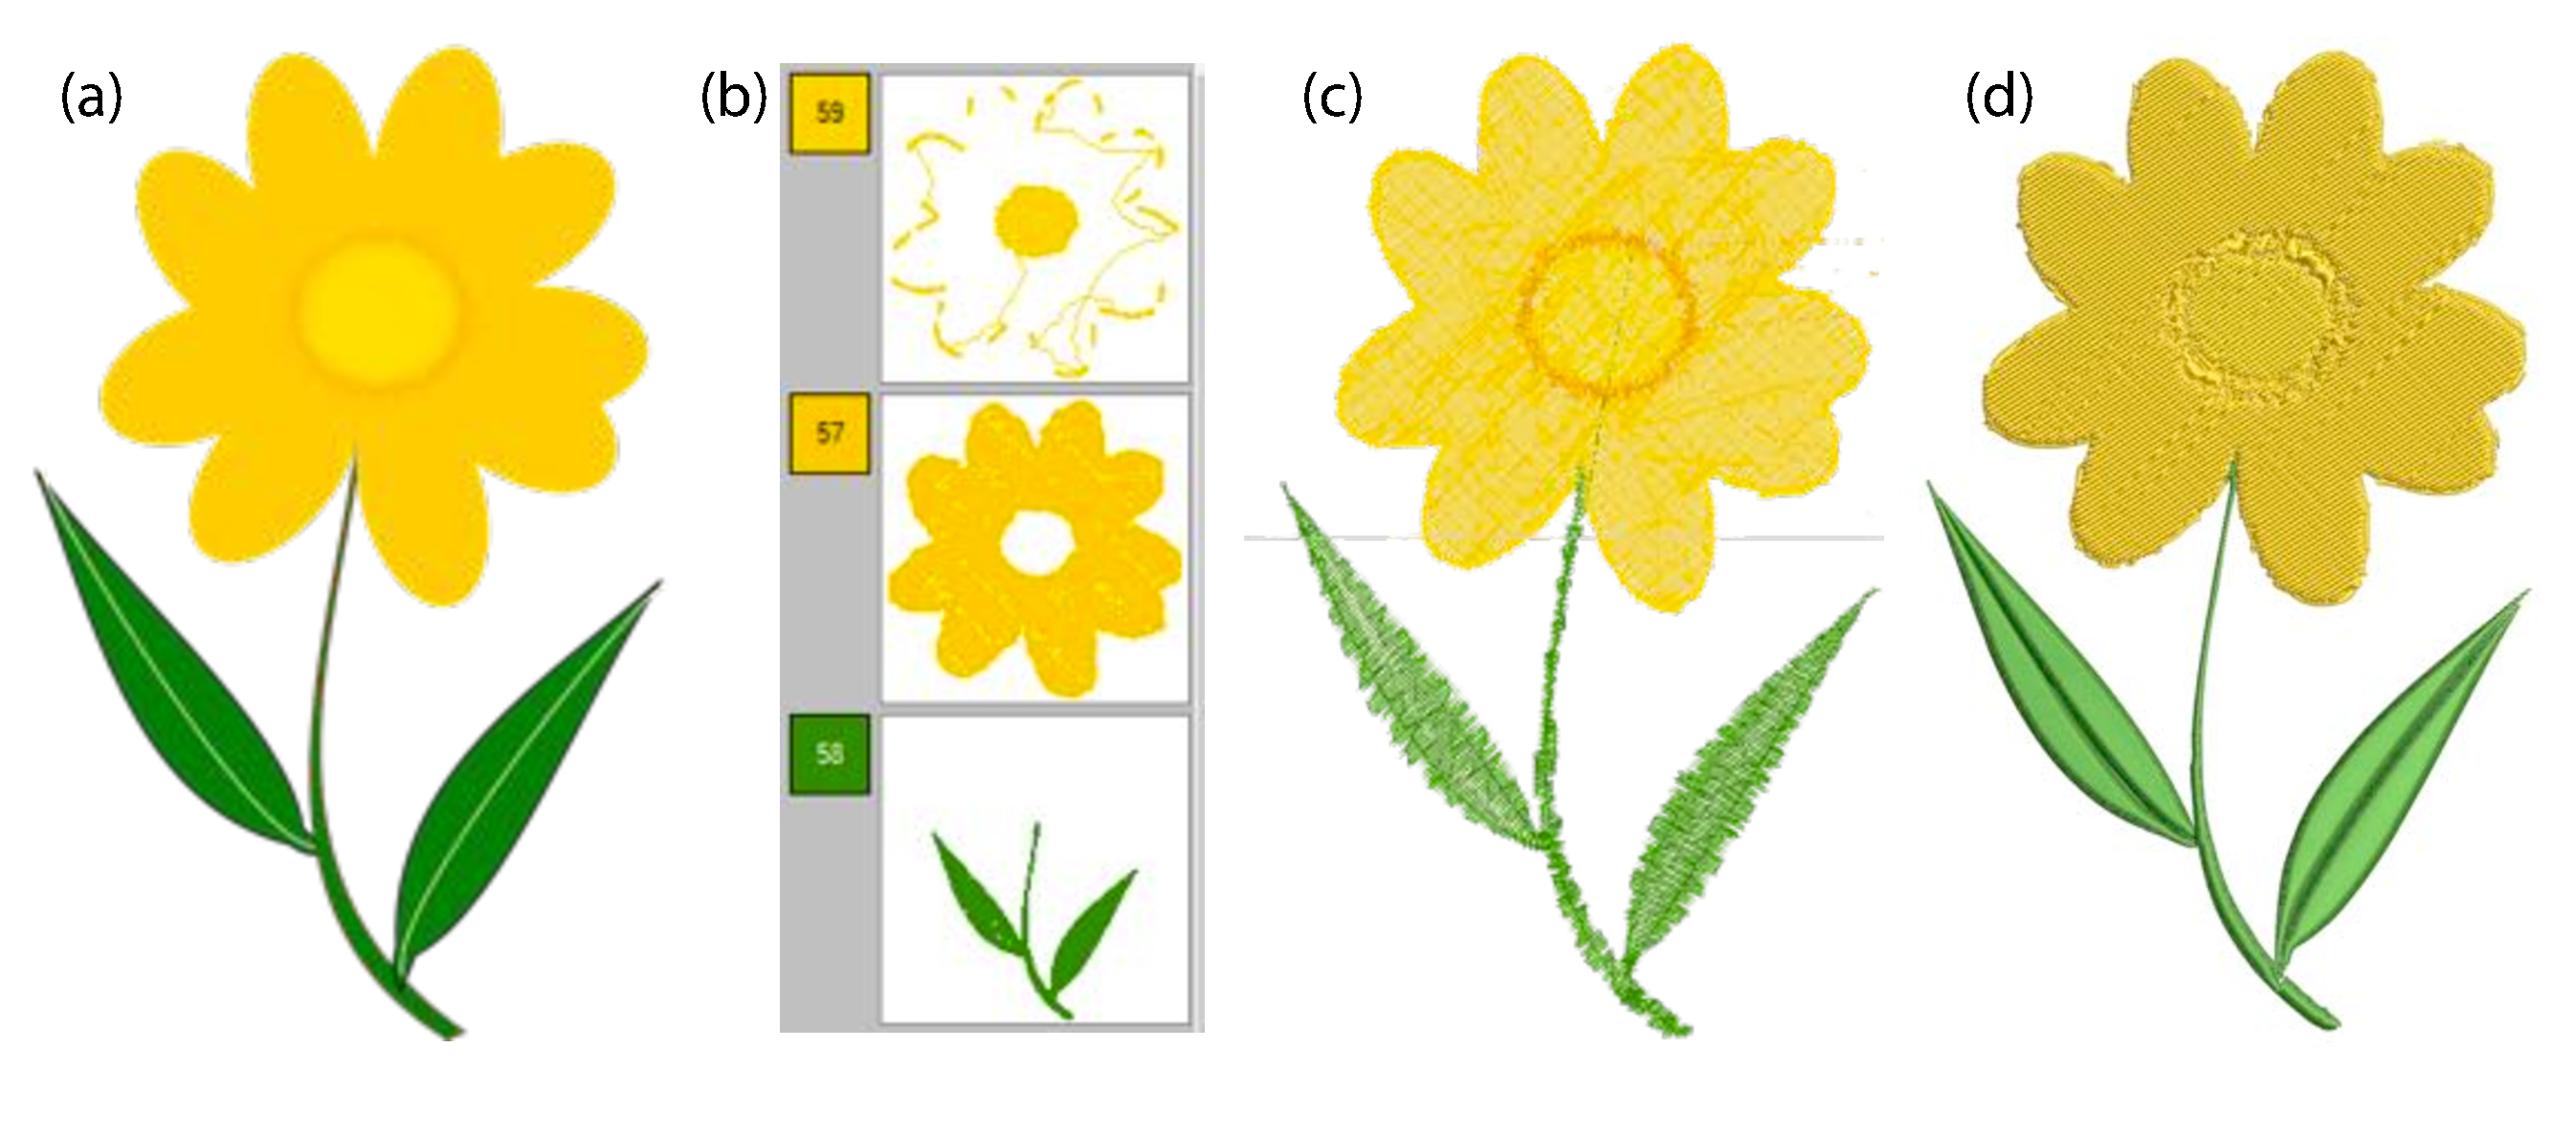
\includegraphics[width=0.9\columnwidth]{figures/EMWorkflow}
  \caption{Image digitization in embroidery software: (a) imported image, (b) separation into color layers with assigned thread colors, (c) generated tool path, (d) final embroidery pattern }~\label{fig:EmbroideryWorkflow}
  \vspace{-2.5em}
\end{figure}

Embroidery machines come with proprietary software that runs on the user's computer. The software transforms color images into embroidery patterns and generates a tool path for the machine. The path dictates how an embroidery hoop moves under the needle. It includes stitch patterns, thread color changes, and jump stitches when traveling between different stitch objects. To optimize tool path generation, embroidery software separates design objects into multiple layers based on color (Fig.\ \ref{fig:EmbroideryWorkflow}). That way, the machine has to stop and prompt the user to manually change thread color less often. Jump stitches also need to be trimmed by hand after embroidery. To reduce these jumps, professional embroidery designers often re-program patterns, manually sequencing stitch objects and individual stitches. 
%Industrial embroidery machines can change thread colors automatically. 
An embroidery machine reads a digitized embroidery pattern from a memory card or a computer connection, recognizes color layers, and stitches them sequentially.

%Virtual hoops help the user position, orient and scale a design relative to physical hoops. 
%Some software tools allow the user to print a design inside a virtual hoop in life-scale to assist the user in aligning the physical hoop on the workpiece fabric.

The internal algorithms that generate a concrete stitching pattern and tool path from a design encode advanced expertise in the mechanical properties of fabrics and threads, not unlike the slicing software turning 3D models into print head tool paths for 3D printers. This complexity is usually kept from the user, but embroidery software still has a relatively steep learning curve, offering a large number of visual design options and specialized tools for manipulating stitch patterns, such as a parametric stitch designer and pull compensation options.
Its user interface assumes a nontrivial amount of expertise in threads, fabrics, embroidery, and the workings of the machine.

\section{Sketch\&Stitch}
Sketch\&Stitch supports a new workflow for creating artistic e-textiles with embroidery machines. The workflow enables users to convert an idea sketched on fabric into an interactive system. It lets users design both artwork and electrical connections in free artistic shapes directly on the work piece, without having to interact with CAD/CAM tools on a computer screen. This allows them to focus on the fabric rather than on the user interface. 
%---> We miss the intelligence of layout software such as Fritzing or Autodesk's Eagle
%---> We miss the preciseness and manipulation of CAD tools
Our workflow utilizes an embroidery machine to take over the laborious tasks in e-textile fabrication---stitching and insulating conductive traces. Yet, it maintains the physical and direct interaction between the user and the work piece during the creative tasks---designing and planning visual and functional patterns. Sketch\&Stitch is thus designed for improvisational design and quick, low-threshold prototyping.
%The workflow with Sketch\&Stitch was developed with designers and makers in mind. 



The Sketch\&Stitch system comprises a smartphone secured on a camera mount above the work surface, a computer, a commercial embroidery machine, and a Bluetooth-connected button (see Fig.\ \ref{fig:UI}). The smartphone runs Sketch\&Stitch (S\&S) mobile app, which captures a picture of the user's sketch and uploads it to a shared cloud folder. The computer runs S\&S PC app and a proprietary embroidery software, DesignerPlus\textsuperscript{\textregistered} v.8. S\&S PC app processes the user's sketch, sends it to the embroidery software to be transformed into embroidery patterns, and finally sends the patterns to the embroidery machine to be stitched. 


Users communicate with Sketch\&Stitch using colored fabric pens and \textcolor{red}{\textit{Circuit Stickers}} on fabric.
%---> Why? Is this the best way of communication? Did we ask users?
To stitch a design, the user places the fabric under the camera mount and presses the wireless button to capture a picture of her sketch. S\&S PC app lets the user verify the processed sketch and tune color detection using a simple slider-based user interface. The user can then view the embroidery patterns via the embroidery machine's touch display. Optionally, the user may use the touch display to manipulate, e.g., scale, mirror translate, or delete patterns. % ...also see the history of transformations
To start stitching, the user threads the needle with the appropriate thread, and presses the start button on the machine.
% ...appropriate thread: conductive or non conductive (colored)
% Google Jacquard offers colored conductive threads for weaving. There is research of dying threads.

Circuit Stickers are symbolic images printed on adhesive paper. 
They are adhered to fabric to represent elements to be added to the circuit during and after embroidery. Sketch\&Stitch supports two types of Circuit Stickers: \textit{Component Stickers} and \textit{Embroidery Stickers}. Component Stickers serve as placeholders for electronic components such as LEDs, motors and speakers, usually on PCBs. Users replace with their hardware counterparts after embroidery is complete, using one of three attachment techniques we describe further below. Embroidery Stickers represent multi-layer custom embroidery patterns required for wire crossings and our textile touch sensors. User remove these stickers after capturing their design via the camera, and our system inserts the required multi-layer patterns in place automatically during the embroidery process.

Circuit Stickers were developed for two reasons: First, the presser foot in embroidery machines only has a clearance of about 1 mm above the fabric, too low for even thin populated PCBs. For comparison, LilyPad PCBs are 0.8 mm thick but in total more than 2 mm high due to the SMD components. This leads to the risk of breaking the needle or machine if they come in contact. Second, we wanted to save the user having to hand-draw the multi-layer embroidery patterns our textile touch sensors etc.\ require. Both kinds of Circuit Stickers help users plan and sketch a circuit with ease and precision. Their adhesive backing allows the user to experiment with different positions  during the design phase, and holds them in place while the fabric is being moved around.


The resulting end-to-end workflow of Sketch\&Stitch is to 1.\ sketch an artwork directly on fabric with a textile pen, 2.\ plan and place Circuit Stickers and draw connections between them, 3.\ capture the design via a camera, 4.\ remove any Embroidery Stickers and stitch the design on the embroidery machine, and finally 5.\ attach the electronics, replacing any Component Stickers. We look at these steps and our solutions for advanced features below.

%We aim to make e-textile creation accessible for emerging designers, hobbyists, crafters, and makers.
%To keep the traditional craft ways of entirely working on the physical workpiece, we developed a pipeline that enables users to sketch the design and plan the circuit directly on fabric. This pipeline 
% Simulating the traditional craft ways of directly interacting with the physical form using tools opens up a range of new creative possibilities [].
%Disconnect between physical and digital: There are numerous sources of variability in textile materials that can make a digital representation unstable, regardless of how good the simulation is.
% More agency and control over the final outcome [Being the Machine: Reconfiguring Agency and Control in Hybrid Fabrication].

\begin{figure}
\centering
  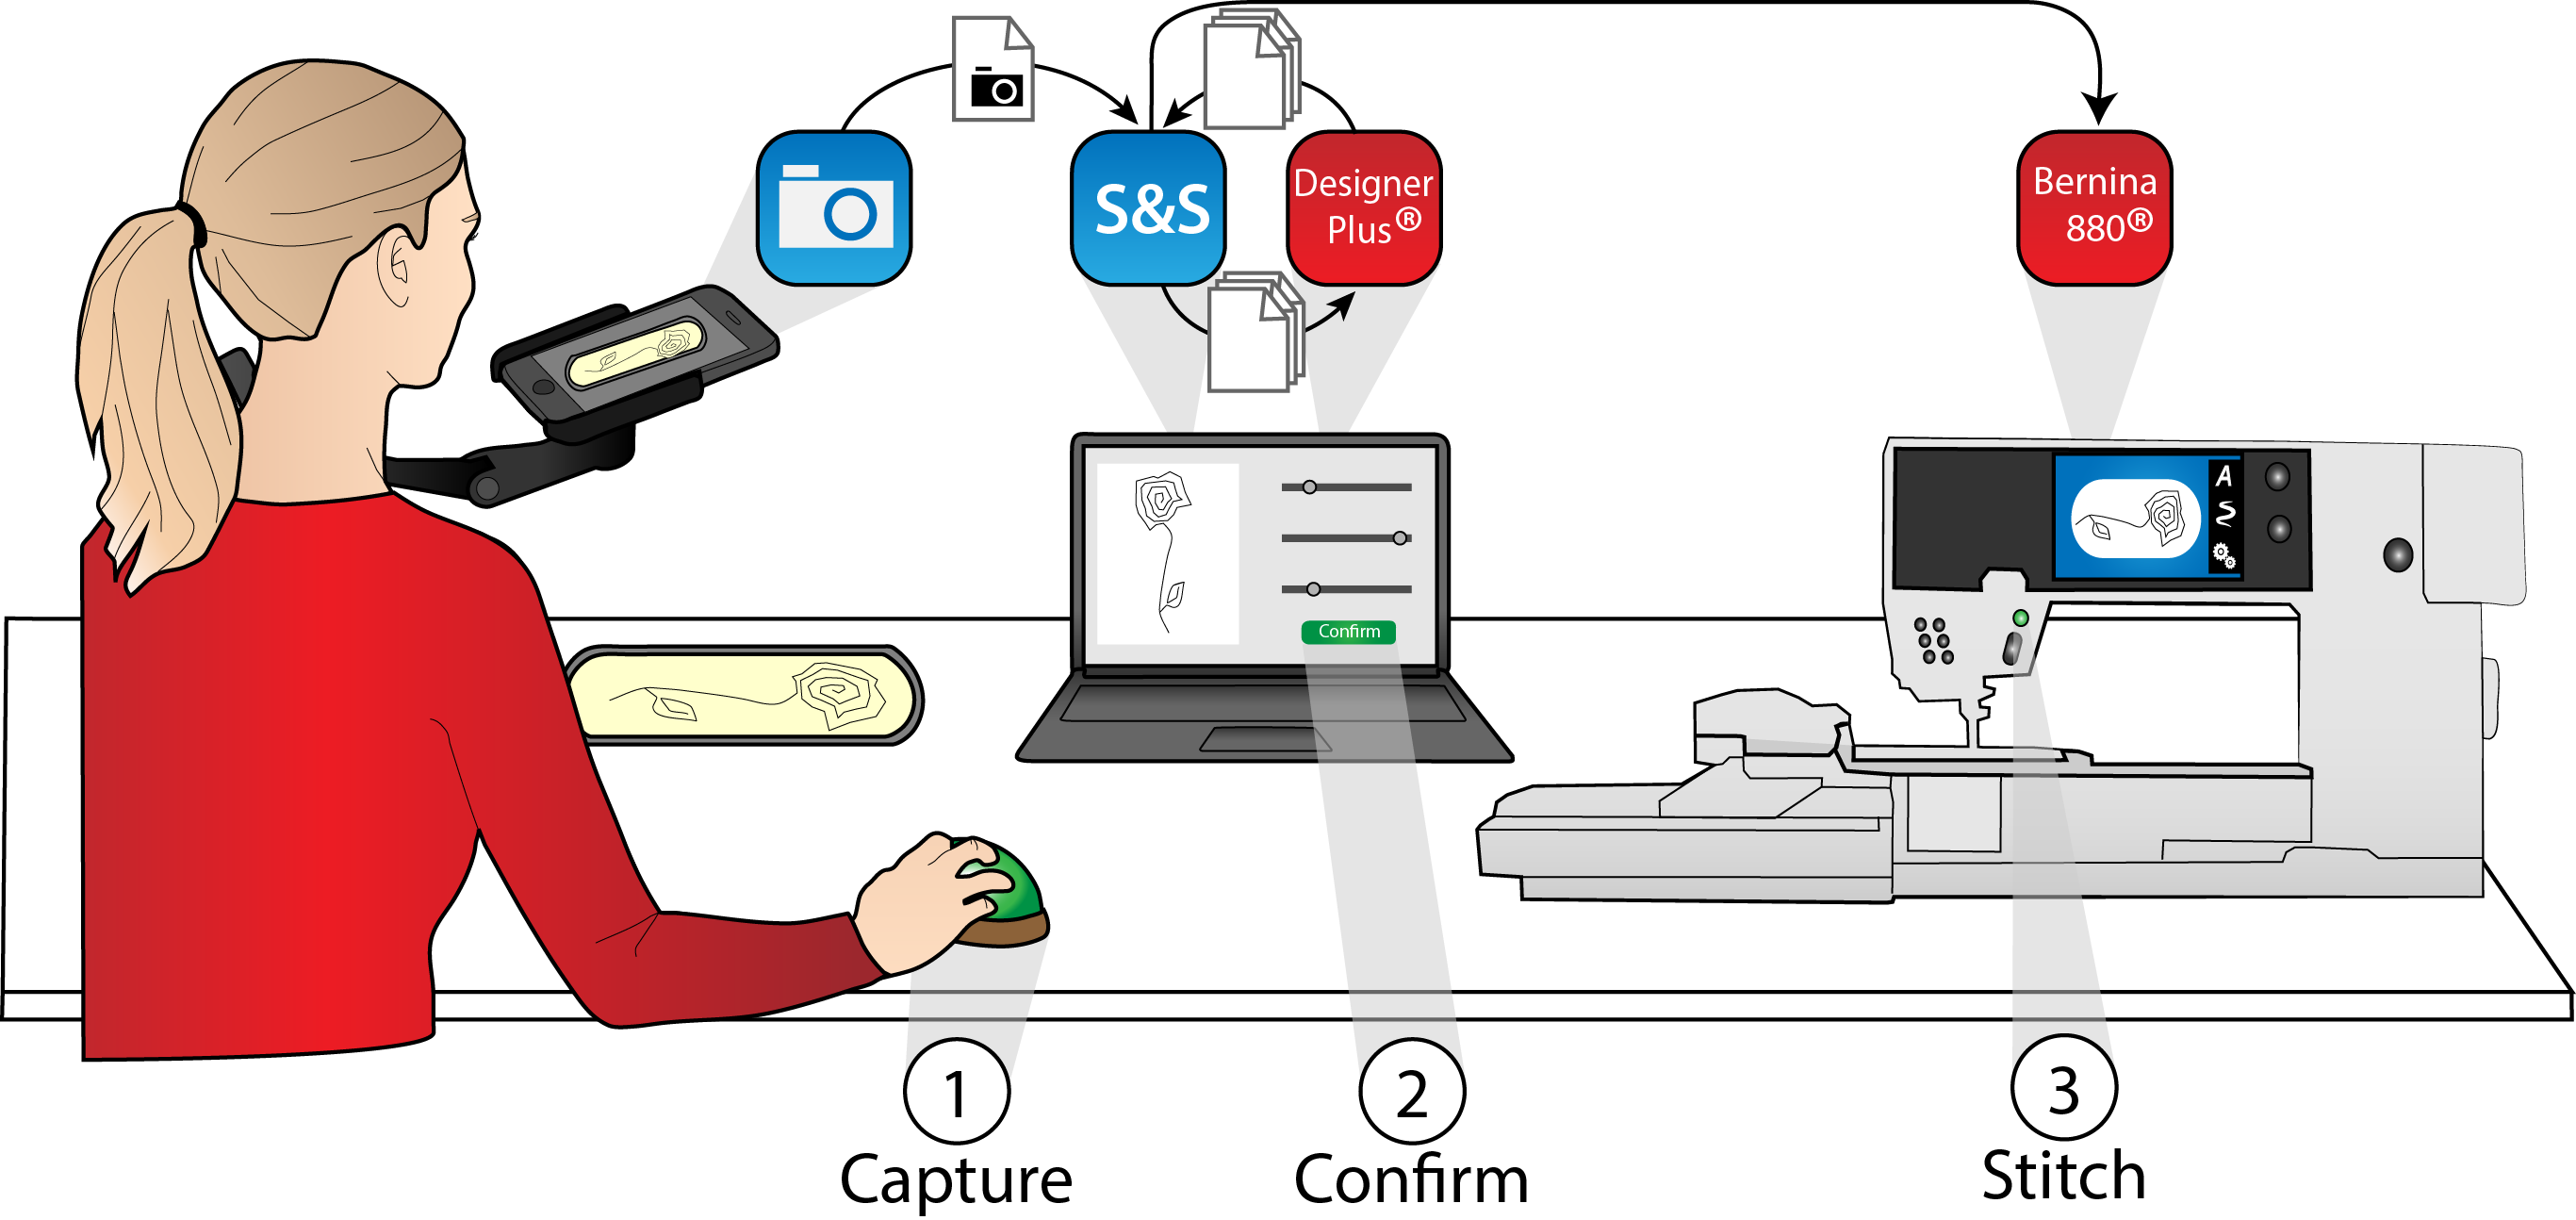
\includegraphics[width=1\columnwidth]{figures/UI.png}
  \caption{The Sketch\&Stitch system and user interface.}~\label{fig:UI}
  \vspace{-1.5em}
\end{figure}


\subsection{Sketching the Design}

%Physical sketching provides users with continuous representation of their workpiece and helps them establish a closer relation with the materials (fabrics, threads, electronics) to better understand their properties and nuances \cite{willis2011interactive}. 
Sketch\&Stitch allows users to draw their designs directly on fabric, enabling them to express themselves freely without the constraints of design applications \cite{landay1995interactive,schweikardt2000digital}. Drawing on fabric is an established art form. It is also used to design patterns for manual embroidery and to mark the placement of buttons, pockets, stitching lines, and other design elements. 

Before sketching on fabric, the user secures it in an embroidery hoop of the desired size. The hoop holds the fabric flat and taut, and frames the design location on the work piece. In our workflow we use water-soluble marking pens to sketch on fabric. The markings of these pens can washed out easily when desired. Our system supports a palette of six pen colors: a \textit{trace color} for drawing electrical traces, an optional \textit{insulation color} for drawing insulated traces, and up to four \textit{art colors} for drawing the artwork. The system preserves the colors white and black, \textit{sticker colors}, for Circuit Stickers. 
%\textcolor{red}{(these are usually not the final \textit{thread colors}, see below).} 
To assign the color palette, the user uses Sketch\&Stitch printable color template. The template consists of six slits, each marked by a name, e.g., trace, insulation, or art, and an AR marker for optical detection. The user places the template on her fabric piece and draws a stroke in each slit using one colored pen. She then captures the template by pressing and holding on the wireless button until she receives auditory feedback from S&S mobile app. %The user repeats this process only if she wants to change the color palette.  

 

%\textcolor{red}{To be able to extend a partly stitched design in subsequent iterations, the user should avoid using thread colors from the color palette.}

Sketch\&Stitch uses colors instead of symbolic sketch annotations for user-system communication to avoid imposing design constraints on freehand sketches, and to keep the design uncluttered. In addition, colors are used to enforce the sequence of pattern execution when communicating with the embroidery machine. For example, in a simple design, the system sequences all objects in \textit{trace color} to be stitched first using conductive thread, followed by objects in each \textit{art color} using non-conductive threads. The number and color of the stitching threads can be chosen during the embroidery process, independently of the color palette. The user simply pauses the embroidery machine every time she wants to switch thread color.


The user can draw her art and circuit in any order.
To \textit{undo} any markings, she erases pen strokes by patting on the fabric with a damp cloth. She can also undo stitched lines using a seam ripper. A design does not need to be complete before it can be stitched. At any point, the user can take a picture of the incomplete sketch, secure the hoop in the embroidery machine, and start the stitching process. This enables her to evaluate and test her design early on, supporting \textit{incremental design}. To use this feature, she should capture a picture of the embroidered fabric before making any new changes. 

\subsection{Adding Electronics}
% The user places Component Stickers on the fabric to serve as placeholders for the electronics hardware to embed in the design. As illustrated above, embroidering with hardware components on the fabric is very challenging for most embroidery machines due to the low (\textasciitilde 1 mm) clearance of the presser foot. %For comparison, LilyPad PCBs are 0.8 mm thick but in total more than 2 mm high due to the SMD components.

\textcolor{red}{Figure \ref{fig:ComponentStickers} shows sample stickers for the LilyPad kit.} Stickers have the same shape, size, and name of their physical counterparts.  
The grooves near the pin holes are added to guide the user and ensure that circuit traces extend under the component and create sufficient contact surface for the attached board. 
%LilyPad components have exposed conductive plates on the top and bottom of the PCB.
The user prints Circuit Stickers from S\&S mobile app on adhesive paper using any printer. Stickers are tinted with \textit{sticker colors}: black and white. To use a sticker, she cuts it out, peels the backing off it, and adheres it to the fabric. %\textit{Embroidery Stickers} representing touch sensor areas can be cut to any desired size. 
Using the \textit{trace color} pen, she then draws circuit traces to connect the stickers. 
%The user may use a vinyl cutter to quickly cut them into shape. 
Component Stickers can be created for any PCB or off-the-shelf components. The only constraint is that they must have a pitch of at least 2.5 mm between their leads (more in section Technical Stitching). The stickers can be reused in later projects.


\begin{figure}
\centering
  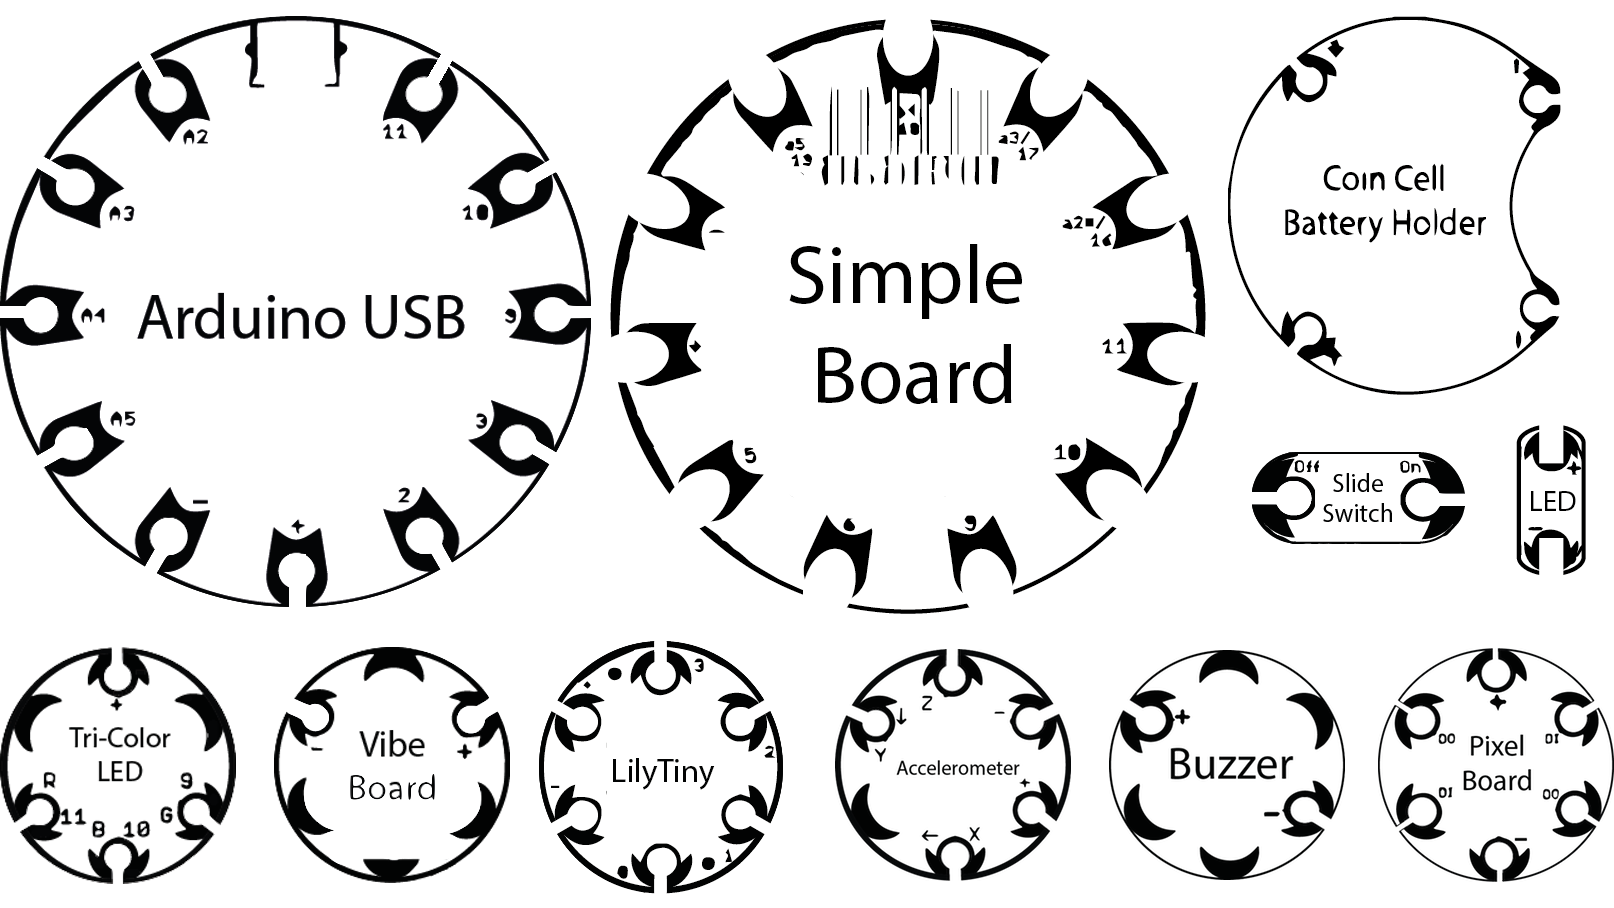
\includegraphics[width=0.9\columnwidth]{figures/ComponentStickers.png}
  \caption{\textcolor{red}{Component Stickers for the Arduino LilyPad electronics kit.}}~\label{fig:ComponentStickers}
  \vspace{-1.5em}
\end{figure}

\subsection{Attaching Electronics}
%We mainly considered sewable components, and components with flat pads on the wrong side of the unit.

%Some stickers include grooves to guide users' traces to ensure reliable electrical connection with the added units. 


After embroidery is complete, the user replaces all Component Stickers with their corresponding hardware components and attaches them to the fabric.
%Sketch\&Stitch simplifies this step by stitching the contact surface  d. 
%Attaching hardware circuit boards and components to fabric is one of the main challenges in e-textiles. Researches have explored several techniques including soldering [], special soldering [], manual sewing [], breads [], ...
We describe three techniques for attaching electronics to fabric. The first uses 3M Electrically Conductive Adhesive Transfer Tape 97033 (Z-tape), a double-sided adhesive that conducts in the $z$ dimension only when compressed. A piece of Z-tape is applied to the back of a component, and the component is aligned to the stitched contact surface on the fabric. Pressing the component down onto the fabric creates connections between pins and contact areas through the Z-Tape. This technique is especially suitable for testing and prototyping a circuit, since it allows for easy removal, but can also be used for final attachment for e-textiles that are not handled much during use.

%We do not know if Z-tape can hold components with legs, we only tested with flat pads.



The second technique uses the embroidery machine. We developed the \textit{LilyStitch}, a custom stitch to attach components with 3 mm diameter pin holes. The stitch is a Single Running stitch, 0.1 mm wide and 9 mm long, made in an M shape, 0.8--1.2 mm wide, with tie-in and tie-off knots on the wider end. The M shape was selected instead of the default line to to create a strong connection and force the tie knots, which require more space than 3 mm, to be stitched outside the pin hole.  
%position of the fabric repeatedly, which can enlarge the hole and weaken the connection, and (b)
%Tie knots need space that 3mm is not encough for them
The length of the LilyStitch accounts for (a) the distance between the center of a pin hole and outer edge of the PCB (\textasciitilde 4 mm), and (b) the distance between needle point and the outer edge of the presser foot (\textasciitilde 5 mm). Shorter distances lead to the presser foot pushing against the edge of the PCB when stitching close to it; longer distances weaken the strength of the stitch.

Figure \ref{fig:LilyStitch} shows a custom embroidery pattern for embroidering a LilyPad Arduino USB board. LilyStitches were sequence-ordered manually to prevent the presser foot from traveling over the board during embroidery. This technique is very reliable and efficient for attaching sewable electronics. However, it requires accurate alignment between the physical component on fabric and the embroidery pattern. If an embroidery machine does not support such accuracy, however, users can stitch part of this pattern directly on fabric, align the component based on the stitches, then restart the embroidery. The physical component should be adhered to the fabric temporarily to keep it from moving. Sketch\&Stitch stores embroidery patterns for stitching LilyPad components on the embroidery machine. The user can access them via the machine's touch display.
%We recommend embroidering the hardware after the art and circuit patterns have been fully embroidered to avoid travel stitches.

\begin{figure}
\centering
  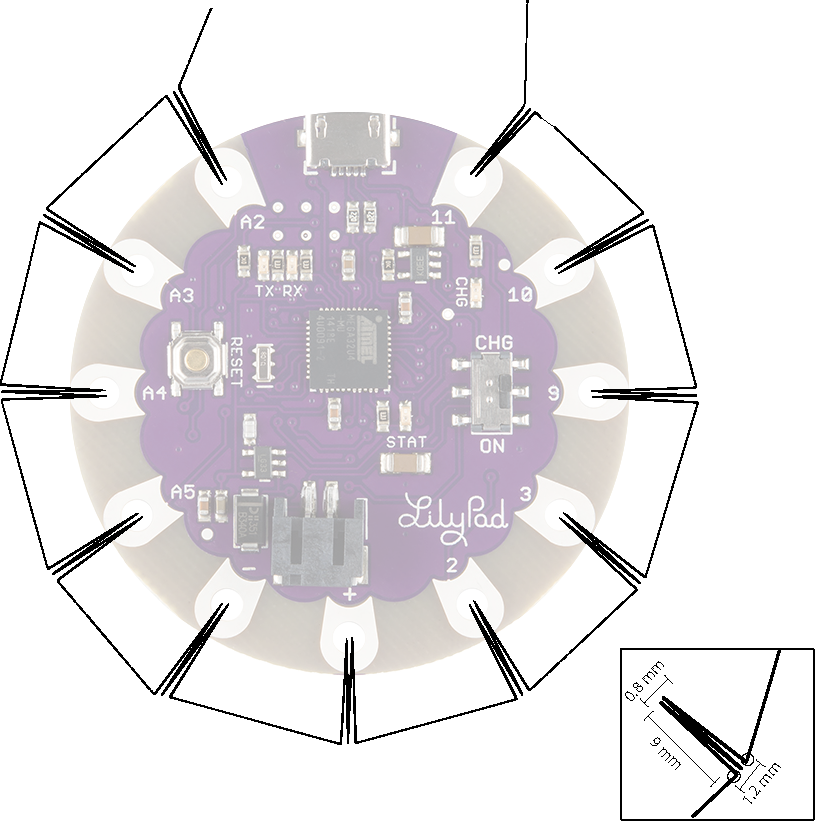
\includegraphics[width=0.8\columnwidth]{figures/LilyStitch}
  \caption{\textcolor{red}{Embroidery pattern of LilyStitches for attaching LilyPad Arduino USB to fabric using an embroidery machine.}}~\label{fig:LilyStitch}
  \vspace{-2em}
\end{figure}

The last technique uses the Button Sewing presser foot in sewing machines. The user has to manually align each pin hole under the presser foot. While this requires some skill, it becomes efficient with practice. Of course, the user can also use the status-quo method of manually sewing into the holes using conductive thread \cite{Buechley:2008:LAU:1357054.1357123}. 
%And part stickers
The results of a sewing machine and manual sewing can be as reliable as using the embroidery machine, but they require more manual labor and time.


\subsection{Insulating circuit traces}
Insulating circuit traces, especially in wearable e-textiles, is paramount for their functionality. %Textiles are flexible materials. 
Exposed traces may come in contact with each other as fabric folds or bends, creating shorts or undesired signals. Buechley et al.\ \cite{Buechley2009} proposed couching---stitching one thread over another---as a natural insulation technique for fabric circuit traces. However, they noted that sewing machines may leave gaps in the couching stitch, making it an unreliable cover for the underlying conductive thread. Computer-controlled embroidery machines are much better at maintaining a consistent couching stitch, making them a perfect fit for this technique. 


To insulate a circuit trace with Sketch\&Stitch, the user draws the trace with the \textit{insulation color} pen. The system detects all objects in this color and creates an \textit{insulation stack}. The stack is composed of two layers, each containing a copy of the objects. Each layer is transformed to an embroidery job: the bottom layer is stitched first using a \textit{trace stitch}, and the top layer is stitched next using a wider \textit{couch stitch}. The \textit{trace stitch} is stitched using conductive thread, and the \textit{couching stitch} using non-conductive thread (more in section Technical Stitching).

While couching circuit traces has functional advantages, it has two pitfalls: It can have a pronounced visual impact on the design due to its thickness, and the build-up of stitches can reduce the flexibility of the base fabric.




 

%\textcolor{red}{The system duplicates all objects in \textit{insulation color}, and stores them in two design layers: the bottom layer, tinted with \textit{trace color}, and the top layer, tinted in \textit{insulation color}. The system uses trace and insulation colors to map stitch types (more in section Technical Considerations) layer colors are used to map to stitch types and to define the sequence of stitching layers in the embroidery software.}
%We describe this process further in Implementation section. 


\subsection{Handling Crossing Traces}
\begin{figure}
\centering
  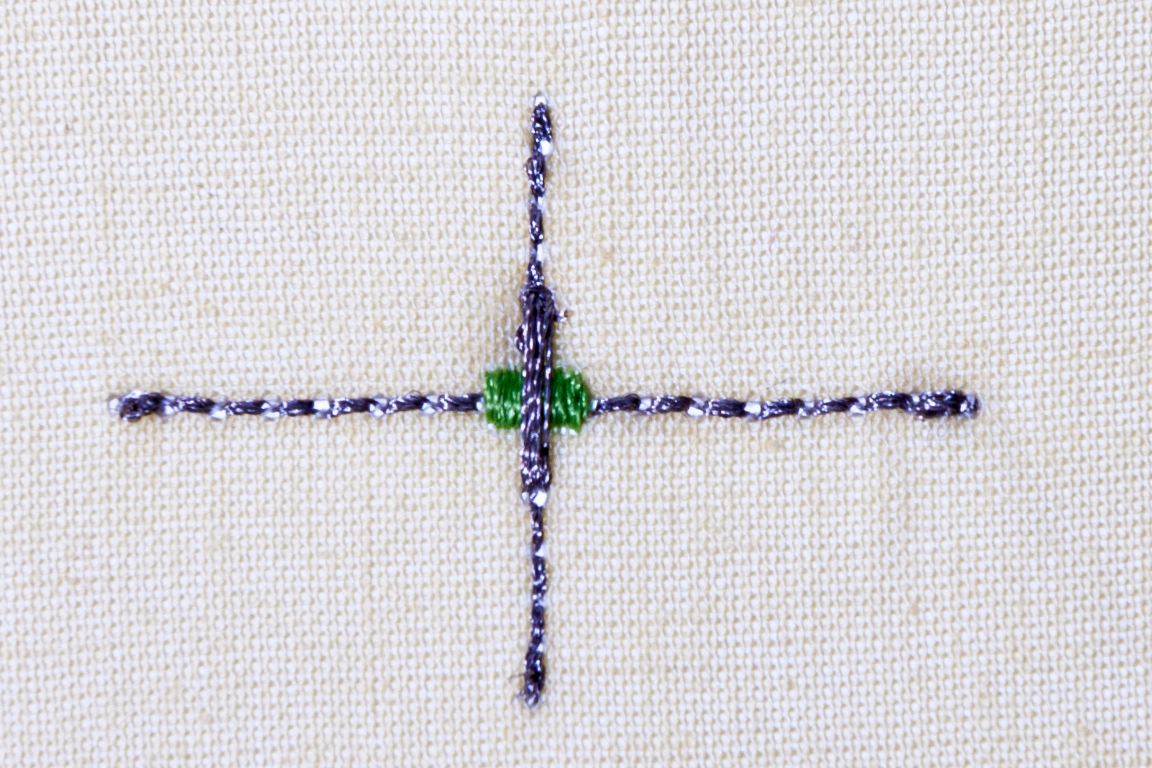
\includegraphics[width=1\columnwidth]{figures/BridgeStitch}
  \caption{Handling crossing traces: (a) shield sticker, (b) three layer embroidery design, (c) shielding using the BridgeStitch.}~\label{fig:BridgeStitch}
  \vspace{-1.5em}
\end{figure}

As the number of circuit elements increases in a design, the need for circuit traces crossing each other becomes inevitable. Dunne et al.\ \cite{Dunne:2012:MEC:2370216.2370348} manipulate the tension of the top and bottom threads to allow two conductive threads to cross without touching. However, from our experience, this technique does not provide fail-safe insulation, especially when pressure is applied to the intersection point. In addition, adjusting the thread tension to be too tight or too loose impairs the strength and appearance of stitches. It may also lead to ``thread birdnesting'', which causes the thread to tangle and the machine to stop.  
%various fabric-thread combinations require different tension settings and changing these settings may affect the appearance and strength of the stitches. 
Instead, Sketch\&Stitch provides users with \textit{Shield Stickers}, Embroidery Stickers to mark trace crossings to insulate on fabric. Embroidery Stickers use include Python AR Makers \ref{} to facilitate optical detection.


To shield an intersection between two traces, the user places a sticker over the intersection point and connects her traces with the traces of the sticker using the \textit{trace color} pen (Fig.\ \ref{fig:BridgeStitch}.a). 
%Self crisscrosses of conductive thread are safe and do not need to be handled.
The system detects the sticker and creates a \textit{shield stack}. The stack is composed of three layers. The bottom layer contains a line segment to connect one of the user's traces. The second layer contains a line segment to couch the bottom segment. The top layer contains a line segment that bridges the user's second trace over the intersection. The layers are stitched using a \textit{trace stitch}, a \textit{couch stitch}, and a \textit{bridge stitch}, respectively. The \textit{bridge stitch} is stitched with conductive thread. It is used to connect two separate traces (up to 9 mm apart) without stitching between them.


\subsection{Adding Interactivity}
% \begin{figure}
% \centering
%   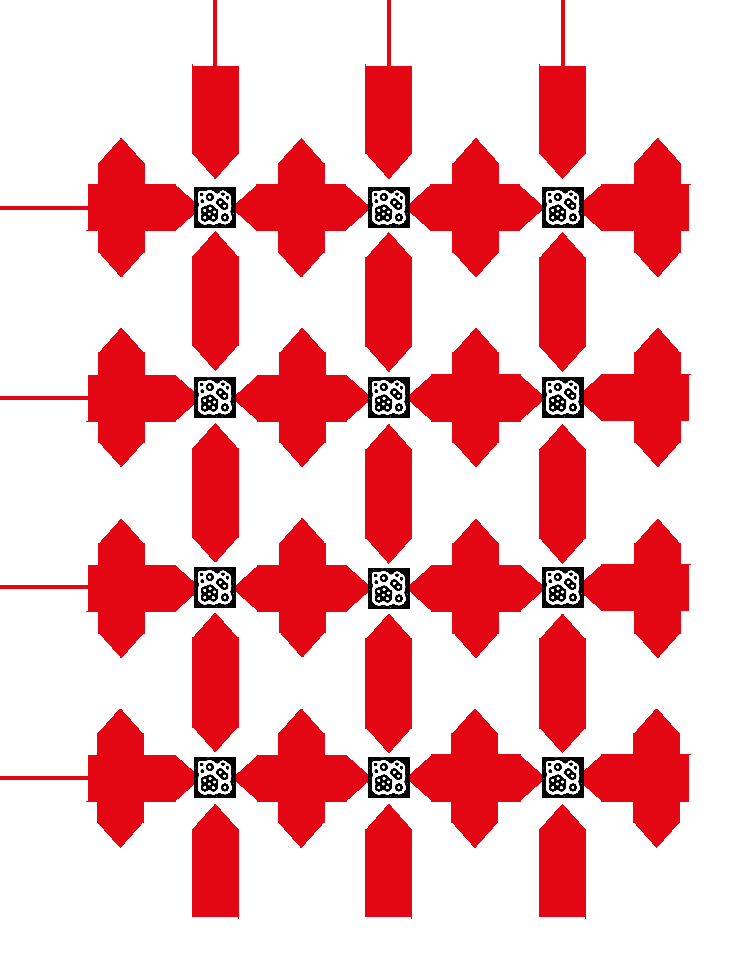
\includegraphics[width=0.6\columnwidth]{figures/RedStickers}
%   \caption{}~\label{fig:RedStickers}
%   \vspace{-2.5em}
% \end{figure}
Besides hardware electronics, users can use \textit{Sensor Stickers}, Embroidery Stickers to add touch sensors made from conductive thread directly onto the fabric. Sketch\&Stitch supports three sensor types: a pushbutton, a slider, and a touchpad.
%actuators, e.g., by couching a shape memory alloy wire, and various touch sensors, as we will demonstrate in this section.

A capacitive pushbutton is the simplest sensor to create, by connecting any segment of conductive thread to a capacitive sensing circuit. The circuit can sense when the user's finger or body is in contact with the thread (touch) or not (no touch). Users can design pushbuttons in any size or shape by simple sketching them with the \textit{trace color}. A resistive pushbutton can be created with two conductive traces 3--4 mm apart that the user bridges when touching, with one trace usually grounded, the other connected to power or a microcontroller pin. Using this simple technique, users can create physical widgets of custom shapes and convert parts of their artwork to touch-enabled surfaces, by using the \textit{trace color} to draw those parts.

%When the user touches the two segments at the same time, a resistive sensing circuit registers a touch.

A slider can be implemented by placing several pushbuttons next to each other. A resistive circuit enables a slider with coarse resolution---the user bridges two neighboring buttons. A capacitive circuit can enable a higher resolution, by interpolating the position of a finger based on the amount of surface area it covers. % and its influence on neighbouring buttons.

% to determine more than one capacitive threshold for a single button. As the user's body comes in contact with more surface o with a capacitive sensor is interacted with by the user, the larger the capacitance will be. 

A matrix of pushbuttons, with each button connected to one IO pin, can be used as a 2D touchpad \cite{hamdan2016grabrics,5387040}. 
%offers the ability to detect all buttons being pressed at the same time, i.e., multi-touch. 
However, a 4$\times$4 touchpad would require 16 pins and traces. This complicates the wiring and may require additional hardware. Instead, using a layout of grid lines with time-multiplexing, as used in capacitive touchscreens, provides a sensor surface area capable of detecting individual touches, simple gestures, and sub-sensor point detection. It requires fewer pins ($4+4=8$ for a 4$\times$4 pad) and less power than scanning individual buttons. 
%However, it cannot support multi-touch. A grid layout can be connected to a capaciiuve or resistive circuit. But due to the low resistivity of the human finger, not all hardware can detect a direct touch. One alternative is to use pinching as an input technique. Hamdan et al. [] were able to detect the location and angle of a pinch on a matrix of resistive textile buttons using simple machine learning algorithms.
%Based on design recommendations from Texas Instruments for capacitive touch sensing with their MSP430 microcontroller\footnote{ www.ti.com/lit/an/slaa363a/slaa363a.pdf}, 
Using the concept of a Shield Sticker, we were able to create a single-layer touchpad sensor. To add a touchpad onto fabric, the user cuts a \textit{Sensor Sticker} in any convex shape, adheres it to the fabric, and draws connecting traces from the sensor's grid lines to pins of a controller using the \textit{trace color} pen. After capturing the design, the user removes the \textit{Sensor Sticker}, and the embroidery machine stitches the sensor pattern in place using the \textit{grid stitch}. The system replaces the Sensor Sticker with a \textit{sensor stack}, which is essentially a grid of \textit{shield stacks}.


To evaluate our single-layer touchpad sensor, we overlaid two pieces of fabric over two 4$\times$4 touchpad sensors, of 7 mm and 9 mm pitch. The fabrics were pre-marked with 9 touch locations each. We measured the error in distance between the touch location on the upper fabric and the measured location on the lower fabric (we used TI MSP430G2553 MCU). We collected a total of 126 readings. The average error in both dimensions for the 7 mm sensors was ($M = , SD = $) and for the 9 mm sensor ($M = , SD = $).  Highest accuracy was achieved when the touch location was aligned with a grid point. Using the 9 mm sensor we can interpolate at least one touch point between any two grid points. Embroidering a 4$\times$4 sensor of 9 mm pitch requires less than 10 minutes.



\begin{figure}
\centering
  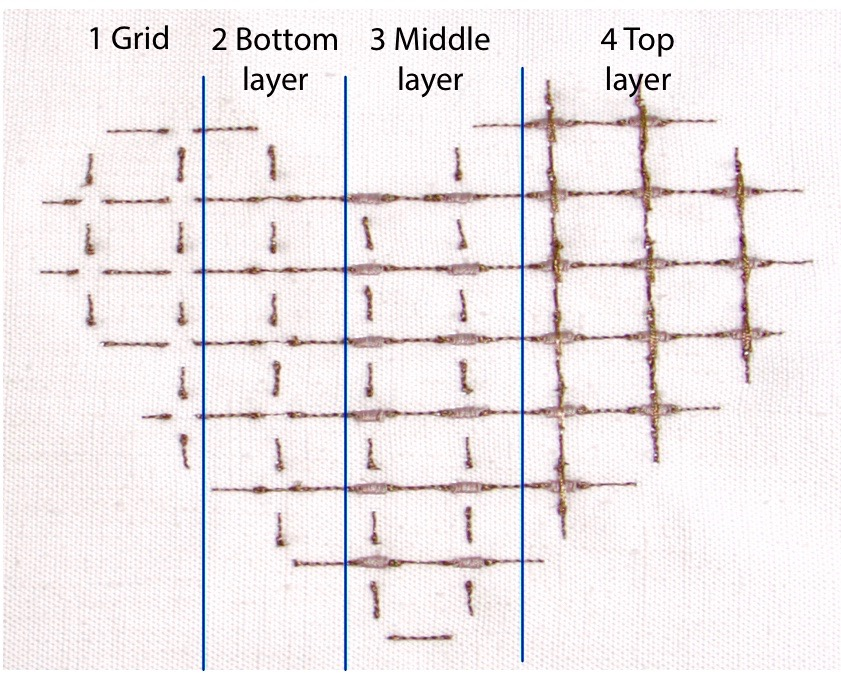
\includegraphics[width=0.7\columnwidth]{figures/heart}
  \caption{Sensor sticker cut into a heart shape and embroidered to show the three design layer.}~\label{fig:Sensor}
  \vspace{-2.5em}
  \end{figure}
  
% To create a sensor in Sketch\&Stitch, the user prints the \textit{Sensor Sticker} on a sheet of adhesive paper, cuts it into the desired shape to create a slider or a touchpad, and sticks it onto the fabric, then draws connecting traces from two sensor grid edges to pins of a controller using the \textit{trace color} marker. After capturing the design, the user removes the \textit{Sensor Sticker}, and the embroidery machine stitches the sensor pattern in place. Fig.\ \ref{fig:Sensor} shows a 2D touchpad at different stages of the embroidery process to show the different layers.

% Electronically speaking, rectangular sensors are the easiest to create that way. The user connects to them at two of their adjacent edges. Other convex shapes require per-line calibration in software to account for the different lengths of grid lines, and concave shapes may also require multiple connections per line if it is interrupted, like the top row in Fig.\ \ref{fig:Sensor}.
% %The grid was designed based on the recommendation of Texas Instruments 


% constructed by “opening up” a capacitor structure so that the
% electric field can be interfered with by a conductive foreign object, in this case, a fingerWhen a conductor, e.g., a finger,
% comes into the area above the open capacitor, the electric field is interfered with causing the
% resulting capacitance to change. The coupling of the conductive finger into the capacitive sensor
% increases the capacitance of the structure beyond the baseline capacitance, the capacitance of
% the sensor with no touch. By continuously measuring the capacitance of the sensor(s) in the
% system and comparing each result to a predetermined baseline capacitance, the system
% microcontroller can determine not only on/off button functions for each sensor element but also
% “amount” of press used for more complex interfaces such as positional sliders. 
% The base capacitance of such a design is affected by stray capacitances on the PCB as well as
% potentially other environmental effects such as temperature and humidity. Therefore, the
% detection system needs to constantly monitor and track this variation for correct comparison to
% touch events. 



 

\subsection{Concealing Traces and Components}
Our system offers five strategies to conceal circuit traces and hardware components in a design: the first is drawing circuit traces to be part of the artwork. The second is drawing circuit traces close to art outlines. 
%The spacing constraint of 2.5 mm need not to be applied between conductive and non-conductive threads. 
While this strategy does not hide the traces, it makes them less obvious. 
%since the width of art stitches is relatively larger than trace stitches.
The third strategy is camouflaging traces by insulating them with a thread color that matches the color of the base fabric \cite{Buechley2009}. Traces will not be hidden completely, but depending on the desired application, this technique may be sufficient to occlude electrical connections. 

The fourth strategy hides hardware components by attaching them to their contact area from the back side of fabric using conductive thread. The fifth strategy allows users to hide fabric circuits and hardware components completely. It uses two layers of fabric: a top layer for sketching the artwork, and a bottom layer for sketching circuit traces and adding Circuit Stickers. The two fabrics are captured and embroidered individually. At the end of embroidery, the user attaches components to the bottom fabric and manually layers the fabrics on top of each other. Capacitive touch sensors will work through a thin top fabric. For components that need to be visible on the surface, such as light sensors and LEDs, the user may cut openings into the top fabric. Another option is attach these parts on the top fabric and use one of the suggested thread-based attachment techniques to connect them to their contact surface on the bottom layer. This technique can also be used to create multi-layer textile circuits \cite{Dunne:2012:MEC:2370216.2370348, 5387040}, with the addition if an insulator like non-conductive fabric, between any two conductive layers. 

%*art colors focrecs the embroidery machine to pause for and wait for the user to chnage thread color. The machine itself can detect color in an image but cannot distigusih thread colors. 


\subsection{Debugging}
Users can debug their designs at three stages in the workflow. After assigning the color palette, S\&S PC app provides the user with a preview of the detected colors on the PC screen. Based on this early feedback, the user chooses to redo color assignment using colors of higher contrast to improve color detection, or start sketching. Similarly, after each capture of the design, our PC app displays a preview of the digitized design that will be transformed to stitches. A mismatch between the design (input) and the preview (output) could be caused by poor lighting, shadows, indistinct strokes, color variability, or other artifacts commonly present in photographed images. Indistinct strokes and color variability occur due to pen jitters over textured fabrics and variable pressures applied while drawing a single stroke, causing the stroke color to vary between darker and lighter shades. Consequently, a trace may appear segmented during color detection, resulting in an open circuit in the final product. To handle these issues, S\&S app offers an optional slider-based interface for manually tuning color detection. Otherwise, the user should perform the proper adjustments directly on the fabric, e.g., remove sources of shadow, or empathizes the strokes, and recapture her design. 


Once the design in transformed to stitches, she sees what the end result will look via the embroidery machine's touch display (WYSIWYG editor). The display offers tools to zoom in-out, duplicate, mirror, translate, etc., the design as a whole but it does not allow the user to change the design on the stitch level. Using this preview, the user can detect the issue of merged lines, which occur when the spacing between two independent lines is less than 0.5 mm (more in section Technical Stitching). The user fixes this by erasing the problematic traces on fabric and re-sketching them apart from each other. Finally, the \textit{incremental design} feature allows her to test the physical design, artwork and circuit, by selectively sketching and stitching parts of it. Optionally, she can use another piece of fabric to stitch the first iteration before committing on the final fabric.


%Limitation, no feedback during sketching, no automatic detection of issues.
%Limitation no more 'adjustment options', e.g., on the stitch level, because they need more experience.
%The history of transformations can be accessed on the embroidery machine.



\section{Walkthrough: Interactive Flower}


We illustrate Sketch\&Stitch's basic design pipeline using the example of an interactive flower that emits light patterns when the user touches one of its leaves. The flower includes 3 LEDs, 1 touch sensor, 1 battery holder, and 1 microcontroller 
%ATmega32U4 Board 
from the LilyPad kit. Fig.\ \ref{fig:Walkthrough} shows the design pipeline.

\begin{figure} 
\centering
  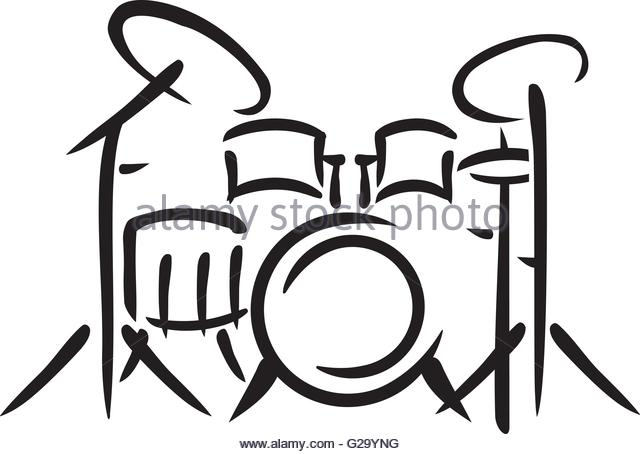
\includegraphics[width=0.9\columnwidth]{figures/Walkthrough}
  \caption{Sketch\&Stitch interaction walkthrough.}~\label{fig:Walkthrough}
  \vspace{-1.5em}
\end{figure}

\subsubsection{Sketching and Placing Circuit Stickers}
At the beginning, the user hoops her fabric and calibrates her marker color palette using the Sketch\&Stitch printed template and smartphone app.
%She places her fabric and markers under the camera mount, and presses  
%prints Circuit Stickers on adhesive paper using her home printer. She cuts the stickers she need for the project---board and pixels. Then, she frames the center of a T-shirt in an embroidery hoop. 
Using a violet \textit{art color} marker, she starts drawing the outline of a flower (\ref{fig:Walkthrough}a). She then places Circuit Stickers inside the flower to estimate their size and location (\ref{fig:Walkthrough}b). Once satisfied with the arrangement, she peels off the stickers' backing and attaches them to the fabric. Using the pink \textit{trace color} marker, she draws circuit traces between the Component Stickers (\ref{fig:Walkthrough}c). She also draws a trace from a pinhole on the controller to the leaf of the flower to create a simple capacitive pushbutton. If she makes a mistake while sketching, she pads a damp cloth on the fabric to erase it.

\subsubsection{Capturing and Embroidering Design}
When she is ready to embroider her design, she presses the button next to the camera mount, and the system captures a picture of the design inside the hoop (\ref{fig:Walkthrough}d). She then secures the hoop in the embroidery machine and uses the embedded display to review the digital embroidery patterns of her design---art and circuit patterns. Since there are no \textit{Embroidery Stickers} to remove in this design, she threads the embroidery needle with conductive thread and starts the embroidery (\ref{fig:Walkthrough}e).  The machine begins embroidering the circuit pattern automatically. Once it is done, it prompts her to change threads. The user picks a non-conductive thread of the color she wants for each part (red for the flower, green for the leave and stem outlines) and starts the machine again. 

% \subsubsection{Debugging}
% After embroidery, the user removes the hoop from the machine, and trims jump stitches. She places the board and pixels over the fabric to verify the alignment of their pins and contact surface. She uses a digital multi-meter to test her traces for any shorts or undesired connections. 

% \subsubsection{Designing Incrementally}
% She cuts a sensor sticker (3$\times$4), and adheres it on fabric. She draws traces from the sensor to the board. Switching to the purple marker, she completes the design of the mandala. She take a picture of the new design, removes the sensor sticker, secures the hoop in the machine, and starts the embroidery machine stitching the sensor and remainder artwork. 

\subsubsection{Attaching Electronics}
After embroidery is complete, the user removes the hoop from the machine, and trims jump stitches using a scissor. She cuts and peels a piece of Z-tape and applies it on the back of her hardware components. Guided by the Circuit Stickers, she determines the location and orientation of each component. She removes the stickers and attaches the matching components to the fabric aligned to their contact surface (\ref{fig:Walkthrough}f). Finally, she inserts a battery into the battery holder and sees her design augmented with a touch-sensitive lightup effect.




%become Finally, the user uses, e.g., Arduino IDE, to program the functionality of her e-textile.



%The user is free to perform this step in any environment since her input is not tracked in real-time. 




\section{Technical Stitching}
Table \ref{tab:Stitches} summarizes the stitches that the Sketch\&Stitch system uses to embroider users designs. For embroidering the artwork, the Satin stitch is used as the \textit{art stitch}. It is important to consider that the width of a sketched line or shape increases by 0--0.2 mm when stitched. This is due to the smoothing algorithm which the embroidery software uses before transforming a digital sketch to embroidery patterns. Thus, gaps that are 0.2 mm wide between adjacent stokes may be filled with stitches. The length of a stitched line increases by 0--0.8 mm for traces and by 0--0.3 mm for insulated traces, based on the length of each stitch. Below, we describe the three empirical tests that we used to determine our system's stitches.



We used a Bernina 880B
%\footnote{www.bernina.com/880}
embroidery machine and its software, DesignerPlus v.8, with Shieldex 117/17 dtex 2-ply silver sewing thread (linear resistance < 30 $\Omega$/cm). 
%http://www.shieldextrading.net/products/yarns-threads/
This thread can carry current for power and signals. The embroidery machine requires two types of thread: a top thread that appears on the surface of the fabric, and a bobbin thread that runs on the back side of the fabric to pull the top thread down. We used conductive thread as a top, or fashion, thread. Embroidery machines give users more control over the shape of the top thread compared to the bobbin. Embroidery is one of the most stressful textile processes for conductive thread \cite{5387040}. This stress leads to thread breaks, which can lead to discontinuities in circuit traces. Thus, we set the stitching speed of the conductive thread to 300-400 stitch/min to reduce the heat and friction that are associated with high speeds. We used needles for metallic thread and a light weight bobbin thread (60 wt).  

\begin{table}[]
\centering
\resizebox{0.47\textwidth}{!}{
\begin{tabular}{lcccc}
\hline
Stitch & Trace & Couch & Bridge & Grid \\ \hline
Type & \multicolumn{1}{l}{Satin} & \multicolumn{1}{l}{Satin} & \multicolumn{1}{l}{Triple Running} & \multicolumn{1}{l}{Triple Running} \\
Length & 0.8 mm & 0.3 mm & 9.0 mm & 1.0 - 2.5 mm \\
Width & 1.0+ mm & 1.8 mm & 1.0 mm & 1.0 mm \\
Shape & \multicolumn{2}{l}{\parbox[l]{0em}{
  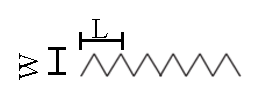
\includegraphics[width=1.1in]{figures/satin_shape}}} & \multicolumn{1}{l}{\parbox[l]{1em}{
  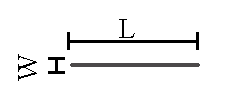
\includegraphics[width=1.1in]{figures/bridge_shape}}} &
  \multicolumn{1}{l}{\parbox[l]{1em}{
  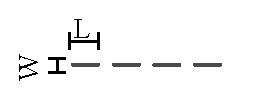
\includegraphics[width=1.1in]{figures/running_shape}}} \\
\hline
\end{tabular}%
}
\caption{ }
\label{tab:Stitches}
\vspace{-1.5em}
\end{table} 


In the following experiments we compared variants of the basic stitch types, Satin and Running. We excluded stitches that are for special purpose or are more decorative. The Satin stitch has a variable width, suitable for outlining lines and filling shapes. Running stitches have a fixed width and are only used for outlines. The tests were conducted on both cotton and linen fabrics. Measurements were taken directly after embroidery, and after one and two weeks of frequent fabric handling. Below, we report the average measurements. 

%Single and and Triple Running are forward stitches, the latter uses three overlapping threads per stitch instead of one.

%Step stitch can also be used as a basic filling stitch, but Satin produces more appealing results.


%---> FW: Need more experiments to understand the effect of thread types (e.g., Madeira), time (aging), base fabric types, on resistance, spacing, and couching 

 \textbf{Resisitivity Test.} Fabric circuits with long electrical connections, traces, drop significantly more voltage, consuming power and limiting the amount of current that can be delivered to components. To determine the best \textit{trace stitch}, we measured the resistance of 30 conductive traces: \textsc{trace length} (5 cm and 10 cm) $\times$ \textsc{stitch type} (Satin, Triple Running, Single Running) $\times$ \textsc{stitch length} (0.4, 0.6, 0.8, 1.0, 2.0 mm), all with minimum width. Table \ref{tab:Resistance} shows sample traces and their average measured resistance. Overall, the resistance of Satin traces was lower than Running traces, independent of \textsc{stitch length}. Satin traces of shorter \textsc{stitch lengths} measure marginally lower resistances. But as the stitch length became shorter, traces became denser. This affects the flexibility of the base fabric, especially if several traces are concentrated in a small area. Longer stitches result in spars traces. Consequently, we chose the Satin stitch of 0.8 mm length as the \textit{trace stitch}. For the \textit{grid stitch} we chose the Triple Running stitch with an adaptable length of 1--2.5 mm. The \textit{grid stitch} is used for stitching insulated traces and sensor grids. As insulated traces will be covered with a \textit{couch stitch} it is essential for them to be flexible. Sensor grids are partially insulated and are concentrated in a small area, using a dense stitch affects sensor flexibility.

\begin{table}[ht] 
\centering
\resizebox{0.47\textwidth}{!}{
\begin{tabular}{lccl} 
  \hline 
  Stitch Type & Stitch Length & Resistance & Sample \hspace{15mm} \\
  \hline  Satin & 0.4 mm & 5--12\Omega & \parbox[c]{1em}{
  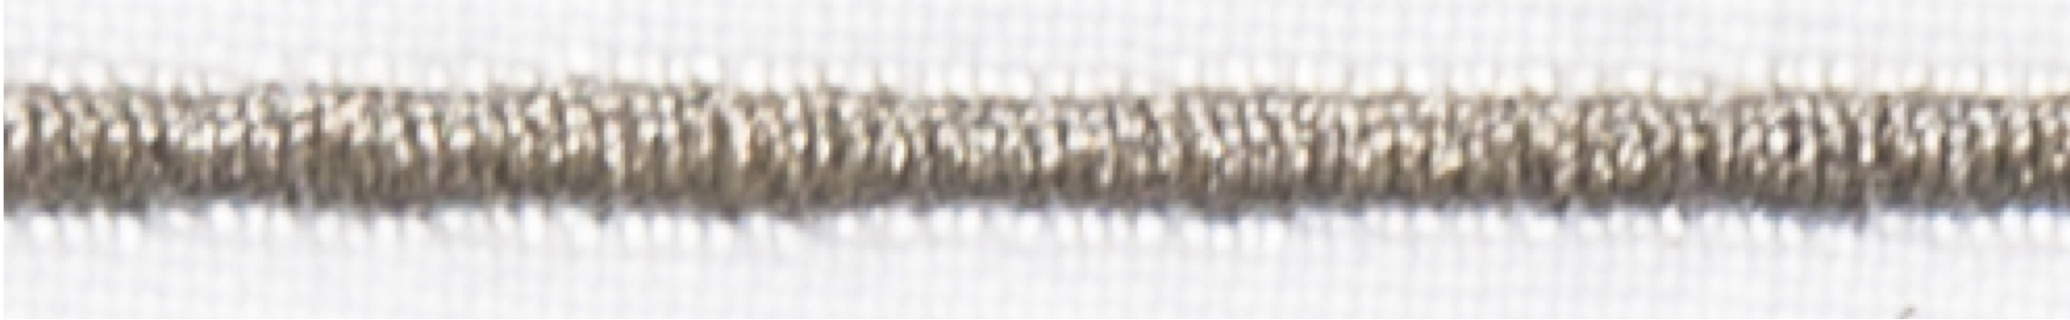
\includegraphics[width=1in]{figures/satin04}} \\
    Satin & 0.6 mm & 12--15 \Omega & \parbox[c]{1em}{
  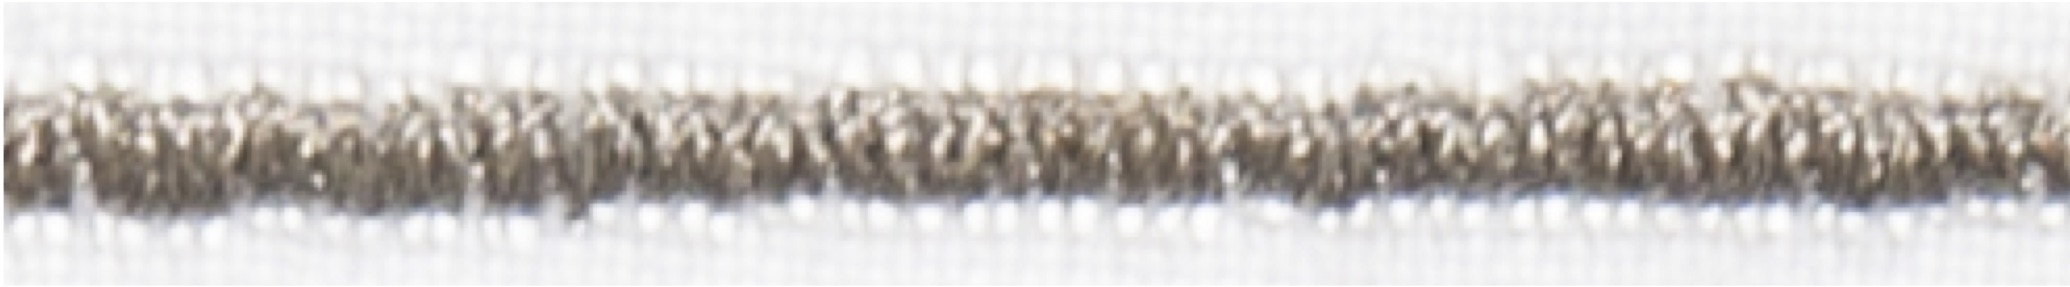
\includegraphics[width=1in]{figures/satin06}} \\
    Satin & 2.0 mm & 14--20 \Omega & \parbox[c]{1em}{
  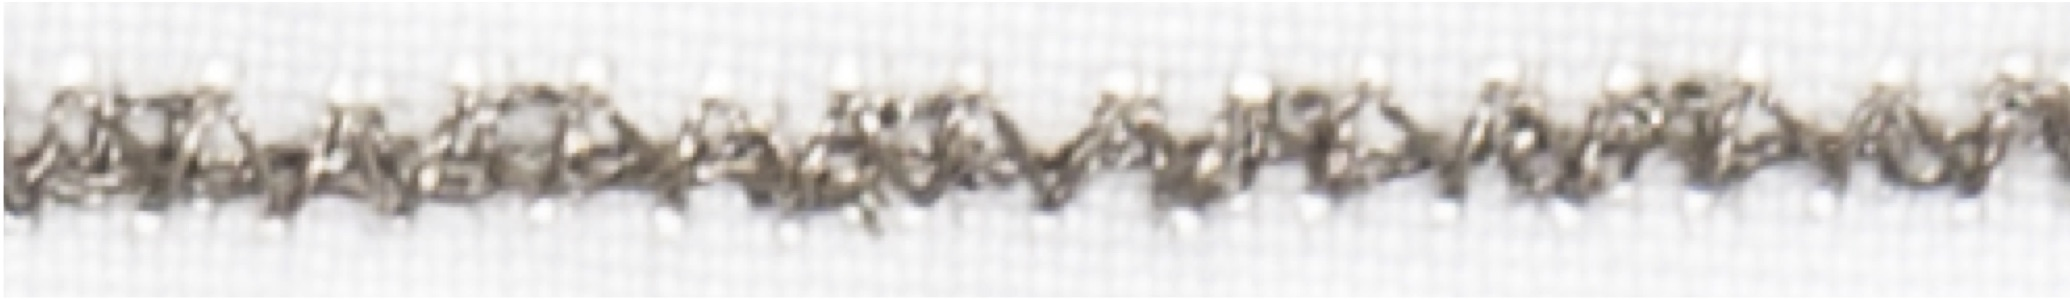
\includegraphics[width=1in]{figures/satin20}} \\
   Triple & 2.0 mm & 27--53 \Omega & \parbox[c]{1em}{
  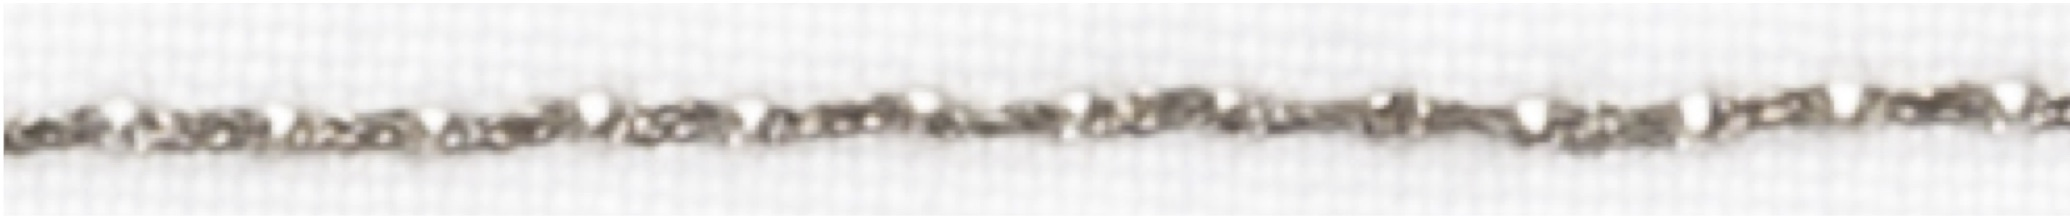
\includegraphics[width=1in]{figures/triple20}} \\
    Single & 2.0 mm & 31--80 \Omega & \parbox[c]{1em}{
  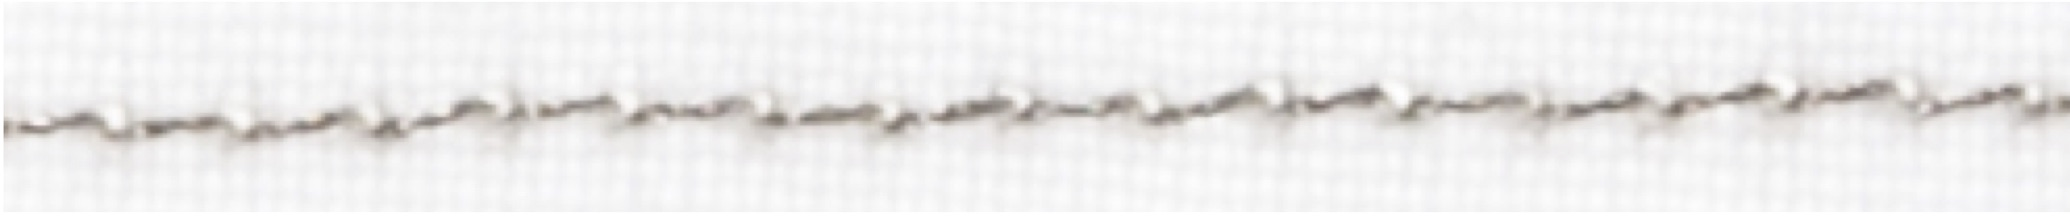
\includegraphics[width=1in]{figures/single20}} \\
   \hline
\end{tabular}
}
\caption{A sample of conductive traces stitched with Satin and Running stitches, and their measured resistance for 5 and 10 cm long segments.}
\label{tab:Resistance}
\vspace{-1.5em}
\end{table}

%Unlike traditional copper wires, conductive threads have relatively high resistances. Resistive threads can be desired for some applications, e.g., \cite{Gowrishankar:2013:PRE:2493988.2494341}. 

%denser stitches increase the number of connections between the conductive fibers that compose a thread, reducing the trace resistance 

\subsection{Spacing Test} 
To evaluate the smallest pitch achievable in our touchpad sensor, we tested the minimum allowed spacing between parallel exposed traces that is immune to undesired connections. We measured for continuity between 6 conductive traces stitched with the \textit{grid stitch}, separated by different \textsc{Spacings} (1.0, 1.5, 2.0, 2.5, 3.0, 3.5 mm). Fraying fibers connected traces at 1.0 and 1.5 mm distances. At 2 mm distance, tie-in and tie-off knots, which are often wider than the trace itself, created undesired contacts on the back of fabric. We conclude that a 2.5 mm is the safe minimum distance between exposed traces. These results are independent of the type, length, and width of a stitch, but may differ for other types of conductive thread with variant fiber lengths. 

\subsection{Insulation Test}
We tested stitches that can be used as a \textit{couch stitch}. Our goal was to find a stitch that prevents undesired connections to occur between insulated and exposed traces even if they come in direct contact with each other, such as in shields and sensors. The most common couch stitch is the Satin (Zigzag) stitch. 
 We tested 16 conductive traces, 10 cm long, stitched with the \textit{grid stitch} and couched with a Satin stitch: \textsc{stitch width} (1.0, 1.4, 1.8, 2.2 mm) $\times$ \textsc{stitch length} (0.7, 0.5, 0.3, 0.1 mm). Each insulated trace was pressed against an exposed conductive trace with four amounts of \textsc{pressure} (1, 5, 15, 30 N) at 5 equidistant points along the trace. We measured for \textit{continuity}. Fig.\ \ref{fig:Insulation} summarizes the results. We found that the Satin stitch of 1.5 mm width and 0.3 mm length insulates a conductive trace on both sides of the fabric while having the least effect on base fabric flexibility. Consequently, two insulated traces can be spaced as close as 2 mm---closer than exposed ones.


\begin{figure}
    \centering
    \resizebox{0.49\textwidth}{!}{
        % Created by tikzDevice version 0.10.1 on 2018-01-06 23:58:38
% !TEX encoding = UTF-8 Unicode
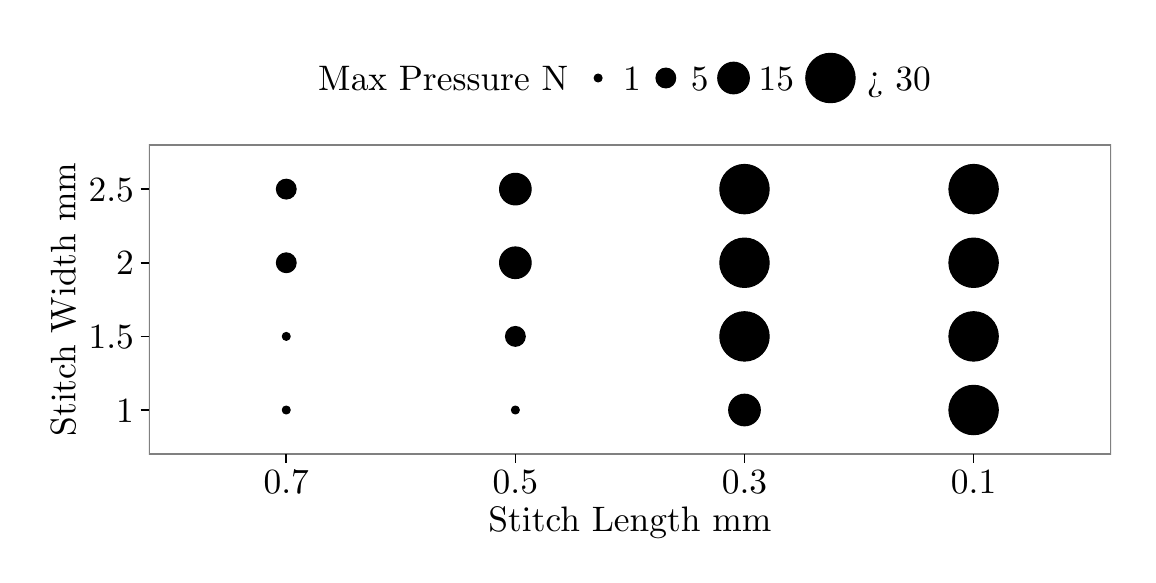
\begin{tikzpicture}[x=1pt,y=1pt]
\definecolor{fillColor}{RGB}{255,255,255}
\path[use as bounding box,fill=fillColor,fill opacity=0.00] (0,0) rectangle (397.48,190.36);
\begin{scope}
\path[clip] (  0.00,  0.00) rectangle (397.48,190.36);
\definecolor{drawColor}{RGB}{255,255,255}
\definecolor{fillColor}{RGB}{255,255,255}

\path[draw=drawColor,line width= 0.6pt,line join=round,line cap=round,fill=fillColor] (  0.00, -0.00) rectangle (397.48,202.36);
\end{scope}
\begin{scope}
\path[clip] ( 43.77, 36.23) rectangle (391.48,147.99);
\definecolor{fillColor}{RGB}{255,255,255}

\path[fill=fillColor] ( 43.77, 36.23) rectangle (391.48,147.99);
\definecolor{drawColor}{RGB}{0,0,0}
\definecolor{fillColor}{RGB}{0,0,0}

\path[draw=drawColor,line width= 0.4pt,line join=round,line cap=round,fill=fillColor] (341.81, 52.20) circle (  8.92);

\path[draw=drawColor,line width= 0.4pt,line join=round,line cap=round,fill=fillColor] (341.81, 78.80) circle (  8.92);

\path[draw=drawColor,line width= 0.4pt,line join=round,line cap=round,fill=fillColor] (341.81,105.41) circle (  8.92);

\path[draw=drawColor,line width= 0.4pt,line join=round,line cap=round,fill=fillColor] (341.81,132.02) circle (  8.92);

\path[draw=drawColor,line width= 0.4pt,line join=round,line cap=round,fill=fillColor] (259.02, 52.20) circle (  5.71);

\path[draw=drawColor,line width= 0.4pt,line join=round,line cap=round,fill=fillColor] (259.02, 78.80) circle (  8.92);

\path[draw=drawColor,line width= 0.4pt,line join=round,line cap=round,fill=fillColor] (259.02,105.41) circle (  8.92);

\path[draw=drawColor,line width= 0.4pt,line join=round,line cap=round,fill=fillColor] (259.02,132.02) circle (  8.92);

\path[draw=drawColor,line width= 0.4pt,line join=round,line cap=round,fill=fillColor] (176.23, 52.20) circle (  1.43);

\path[draw=drawColor,line width= 0.4pt,line join=round,line cap=round,fill=fillColor] (176.23, 78.80) circle (  3.57);

\path[draw=drawColor,line width= 0.4pt,line join=round,line cap=round,fill=fillColor] (176.23,105.41) circle (  5.71);

\path[draw=drawColor,line width= 0.4pt,line join=round,line cap=round,fill=fillColor] (176.23,132.02) circle (  5.71);

\path[draw=drawColor,line width= 0.4pt,line join=round,line cap=round,fill=fillColor] ( 93.44, 52.20) circle (  1.43);

\path[draw=drawColor,line width= 0.4pt,line join=round,line cap=round,fill=fillColor] ( 93.44, 78.80) circle (  1.43);

\path[draw=drawColor,line width= 0.4pt,line join=round,line cap=round,fill=fillColor] ( 93.44,105.41) circle (  3.57);

\path[draw=drawColor,line width= 0.4pt,line join=round,line cap=round,fill=fillColor] ( 93.44,132.02) circle (  3.57);
\definecolor{drawColor}{gray}{0.50}

\path[draw=drawColor,line width= 0.6pt,line join=round,line cap=round] ( 43.77, 36.23) rectangle (391.48,147.99);
\end{scope}
\begin{scope}
\path[clip] (  0.00,  0.00) rectangle (397.48,202.36);
\definecolor{drawColor}{RGB}{0,0,0}

\node[text=drawColor,anchor=base east,inner sep=0pt, outer sep=0pt, scale=  1.28] at ( 38.37, 47.79) {1};

\node[text=drawColor,anchor=base east,inner sep=0pt, outer sep=0pt, scale=  1.28] at ( 38.37, 74.40) {1.5};

\node[text=drawColor,anchor=base east,inner sep=0pt, outer sep=0pt, scale=  1.28] at ( 38.37,101.01) {2};

\node[text=drawColor,anchor=base east,inner sep=0pt, outer sep=0pt, scale=  1.28] at ( 38.37,127.61) {2.5};
\end{scope}
\begin{scope}
\path[clip] (  0.00,  0.00) rectangle (397.48,202.36);
\definecolor{drawColor}{RGB}{0,0,0}

\path[draw=drawColor,line width= 0.6pt,line join=round] ( 40.77, 52.20) --
	( 43.77, 52.20);

\path[draw=drawColor,line width= 0.6pt,line join=round] ( 40.77, 78.80) --
	( 43.77, 78.80);

\path[draw=drawColor,line width= 0.6pt,line join=round] ( 40.77,105.41) --
	( 43.77,105.41);

\path[draw=drawColor,line width= 0.6pt,line join=round] ( 40.77,132.02) --
	( 43.77,132.02);
\end{scope}
\begin{scope}
\path[clip] (  0.00,  0.00) rectangle (397.48,202.36);
\definecolor{drawColor}{RGB}{0,0,0}

\path[draw=drawColor,line width= 0.6pt,line join=round] ( 93.44, 33.23) --
	( 93.44, 36.23);

\path[draw=drawColor,line width= 0.6pt,line join=round] (176.23, 33.23) --
	(176.23, 36.23);

\path[draw=drawColor,line width= 0.6pt,line join=round] (259.02, 33.23) --
	(259.02, 36.23);

\path[draw=drawColor,line width= 0.6pt,line join=round] (341.81, 33.23) --
	(341.81, 36.23);
\end{scope}
\begin{scope}
\path[clip] (  0.00,  0.00) rectangle (397.48,202.36);
\definecolor{drawColor}{RGB}{0,0,0}

\node[text=drawColor,anchor=base,inner sep=0pt, outer sep=0pt, scale=  1.28] at ( 93.44, 22.02) {0.7};

\node[text=drawColor,anchor=base,inner sep=0pt, outer sep=0pt, scale=  1.28] at (176.23, 22.02) {0.5};

\node[text=drawColor,anchor=base,inner sep=0pt, outer sep=0pt, scale=  1.28] at (259.02, 22.02) {0.3};

\node[text=drawColor,anchor=base,inner sep=0pt, outer sep=0pt, scale=  1.28] at (341.81, 22.02) {0.1};
\end{scope}
\begin{scope}
\path[clip] (  0.00,  0.00) rectangle (397.48,202.36);
\definecolor{drawColor}{RGB}{0,0,0}

\node[text=drawColor,anchor=base,inner sep=0pt, outer sep=0pt, scale=  1.28] at (217.63,  8.40) {Stitch Length mm};
\end{scope}
\begin{scope}
\path[clip] (  0.00,  0.00) rectangle (397.48,202.36);
\definecolor{drawColor}{RGB}{0,0,0}

\node[text=drawColor,rotate= 90.00,anchor=base,inner sep=0pt, outer sep=0pt, scale=  1.28] at ( 17.22, 92.11) {Stitch Width mm};
\end{scope}
\begin{scope}
\path[clip] (  0.00,  0.00) rectangle (397.48,202.36);
\definecolor{fillColor}{RGB}{255,255,255}

\path[fill=fillColor] (100.70,156.52) rectangle (334.55,187.82);
\end{scope}
\begin{scope}
\path[clip] (  0.00,  0.00) rectangle (397.48,202.36);
\definecolor{drawColor}{RGB}{0,0,0}

\node[text=drawColor,anchor=base west,inner sep=0pt, outer sep=0pt, scale=  1.28] at (104.97,167.76) {Max Pressure N};
\end{scope}
\begin{scope}
\path[clip] (  0.00,  0.00) rectangle (397.48,202.36);
\definecolor{drawColor}{RGB}{255,255,255}
\definecolor{fillColor}{RGB}{255,255,255}

\path[draw=drawColor,line width= 0.6pt,line join=round,line cap=round,fill=fillColor] (198.90,160.79) rectangle (213.36,183.55);
\end{scope}
\begin{scope}
\path[clip] (  0.00,  0.00) rectangle (397.48,202.36);
\definecolor{drawColor}{RGB}{0,0,0}
\definecolor{fillColor}{RGB}{0,0,0}

\path[draw=drawColor,line width= 0.4pt,line join=round,line cap=round,fill=fillColor] (206.13,172.17) circle (  1.43);
\end{scope}
\begin{scope}
\path[clip] (  0.00,  0.00) rectangle (397.48,202.36);
\definecolor{drawColor}{RGB}{255,255,255}
\definecolor{fillColor}{RGB}{255,255,255}

\path[draw=drawColor,line width= 0.6pt,line join=round,line cap=round,fill=fillColor] (223.37,160.79) rectangle (237.82,183.55);
\end{scope}
\begin{scope}
\path[clip] (  0.00,  0.00) rectangle (397.48,202.36);
\definecolor{drawColor}{RGB}{0,0,0}
\definecolor{fillColor}{RGB}{0,0,0}

\path[draw=drawColor,line width= 0.4pt,line join=round,line cap=round,fill=fillColor] (230.60,172.17) circle (  3.57);
\end{scope}
\begin{scope}
\path[clip] (  0.00,  0.00) rectangle (397.48,202.36);
\definecolor{drawColor}{RGB}{255,255,255}
\definecolor{fillColor}{RGB}{255,255,255}

\path[draw=drawColor,line width= 0.6pt,line join=round,line cap=round,fill=fillColor] (247.84,160.79) rectangle (262.29,183.55);
\end{scope}
\begin{scope}
\path[clip] (  0.00,  0.00) rectangle (397.48,202.36);
\definecolor{drawColor}{RGB}{0,0,0}
\definecolor{fillColor}{RGB}{0,0,0}

\path[draw=drawColor,line width= 0.4pt,line join=round,line cap=round,fill=fillColor] (255.06,172.17) circle (  5.71);
\end{scope}
\begin{scope}
\path[clip] (  0.00,  0.00) rectangle (397.48,202.36);
\definecolor{drawColor}{RGB}{255,255,255}
\definecolor{fillColor}{RGB}{255,255,255}

\path[draw=drawColor,line width= 0.6pt,line join=round,line cap=round,fill=fillColor] (278.70,160.79) rectangle (301.46,183.55);
\end{scope}
\begin{scope}
\path[clip] (  0.00,  0.00) rectangle (397.48,202.36);
\definecolor{drawColor}{RGB}{0,0,0}
\definecolor{fillColor}{RGB}{0,0,0}

\path[draw=drawColor,line width= 0.4pt,line join=round,line cap=round,fill=fillColor] (290.08,172.17) circle (  8.92);
\end{scope}
\begin{scope}
\path[clip] (  0.00,  0.00) rectangle (397.48,202.36);
\definecolor{drawColor}{RGB}{0,0,0}

\node[text=drawColor,anchor=base west,inner sep=0pt, outer sep=0pt, scale=  1.28] at (215.17,167.76) {1};
\end{scope}
\begin{scope}
\path[clip] (  0.00,  0.00) rectangle (397.48,202.36);
\definecolor{drawColor}{RGB}{0,0,0}

\node[text=drawColor,anchor=base west,inner sep=0pt, outer sep=0pt, scale=  1.28] at (239.63,167.76) {5};
\end{scope}
\begin{scope}
\path[clip] (  0.00,  0.00) rectangle (397.48,202.36);
\definecolor{drawColor}{RGB}{0,0,0}

\node[text=drawColor,anchor=base west,inner sep=0pt, outer sep=0pt, scale=  1.28] at (264.10,167.76) {15};
\end{scope}
\begin{scope}
\path[clip] (  0.00,  0.00) rectangle (397.48,202.36);
\definecolor{drawColor}{RGB}{0,0,0}

\node[text=drawColor,anchor=base west,inner sep=0pt, outer sep=0pt, scale=  1.28] at (303.27,167.76) {> 30};
\end{scope}
\end{tikzpicture}

    }
    \caption{}
    \label{fig:Insulation}
    \vspace{-1.5em}
\end{figure}

 


\subfile{Implementation}




\section{Example Applications Created By an Artist} % and Emerging Design processes
To reveal some of the early opportunities and challenges of Sketch\&Stitch workflow, we invited a hobbyist artist with a technical background (female, 24 years old) to create artworks using our system. Since the Sketch\&Stitch system was not designed with walk-up and use in mind, we asked the artist to work with it over the course of three days. In the first day, the artist received a twenty-minute introduction of our system. For the next four hours, she explored the system in practice, sketching and stitching simple shapes and basic electrical circuits. In the following two days, the artist spent a total of 10 hours of unrestricted creative work. We observed and documented the artist's process and artifacts, conducted 2 unrestricted interviews (day 1 and 2), a structured interview (day 3), and finally a retrospective study with the artist and researcher reviewing photos of her progress.

Below, we describe three unique artworks that were developed by the artist. The artist used the LilyPad hardware components and the Arduino IDE to program them. We follow this with a brief summary of the user's feedback and  initial insights. 

%we interviewed her to understand the design process that emerged while using our system. We describe these processes after the examples.


\subsection{Wearable Mandala}
\begin{figure} [h!]
\centering
  \includegraphics[width=1\columnwidth]{figures/Mandala} 
  \caption{Example 1: The Wearable Mandala. Size 150$\times$150 mm, 20,000 stitches, 4 thread changes, 28 minutes stitch duration.}~\label{fig:Mandala}
  \vspace{-1.5em}
\end{figure}
The first example is a wearable application. The artist sketched a mandal on a white cotton t-shirt using 3 art colors. Her electrical circuit consisted of 8 LEDs, a microcontroller, and a hidden battery. The artist used the outlines of the mandala to conceal the circuit traces (first concealing strategy). She embroidered frames to house the hardware components, and a contact surface for the battery holder. The battery holder was attached to the contact surface from the back side of the fabric to hide it (second concealing strategy). The mandala lit up in different patterns based on a set of timers. 
%every time she received a message on her smartphone.  



\subsection{Interactive Desk Mat}
\begin{figure} [h!]
\centering
  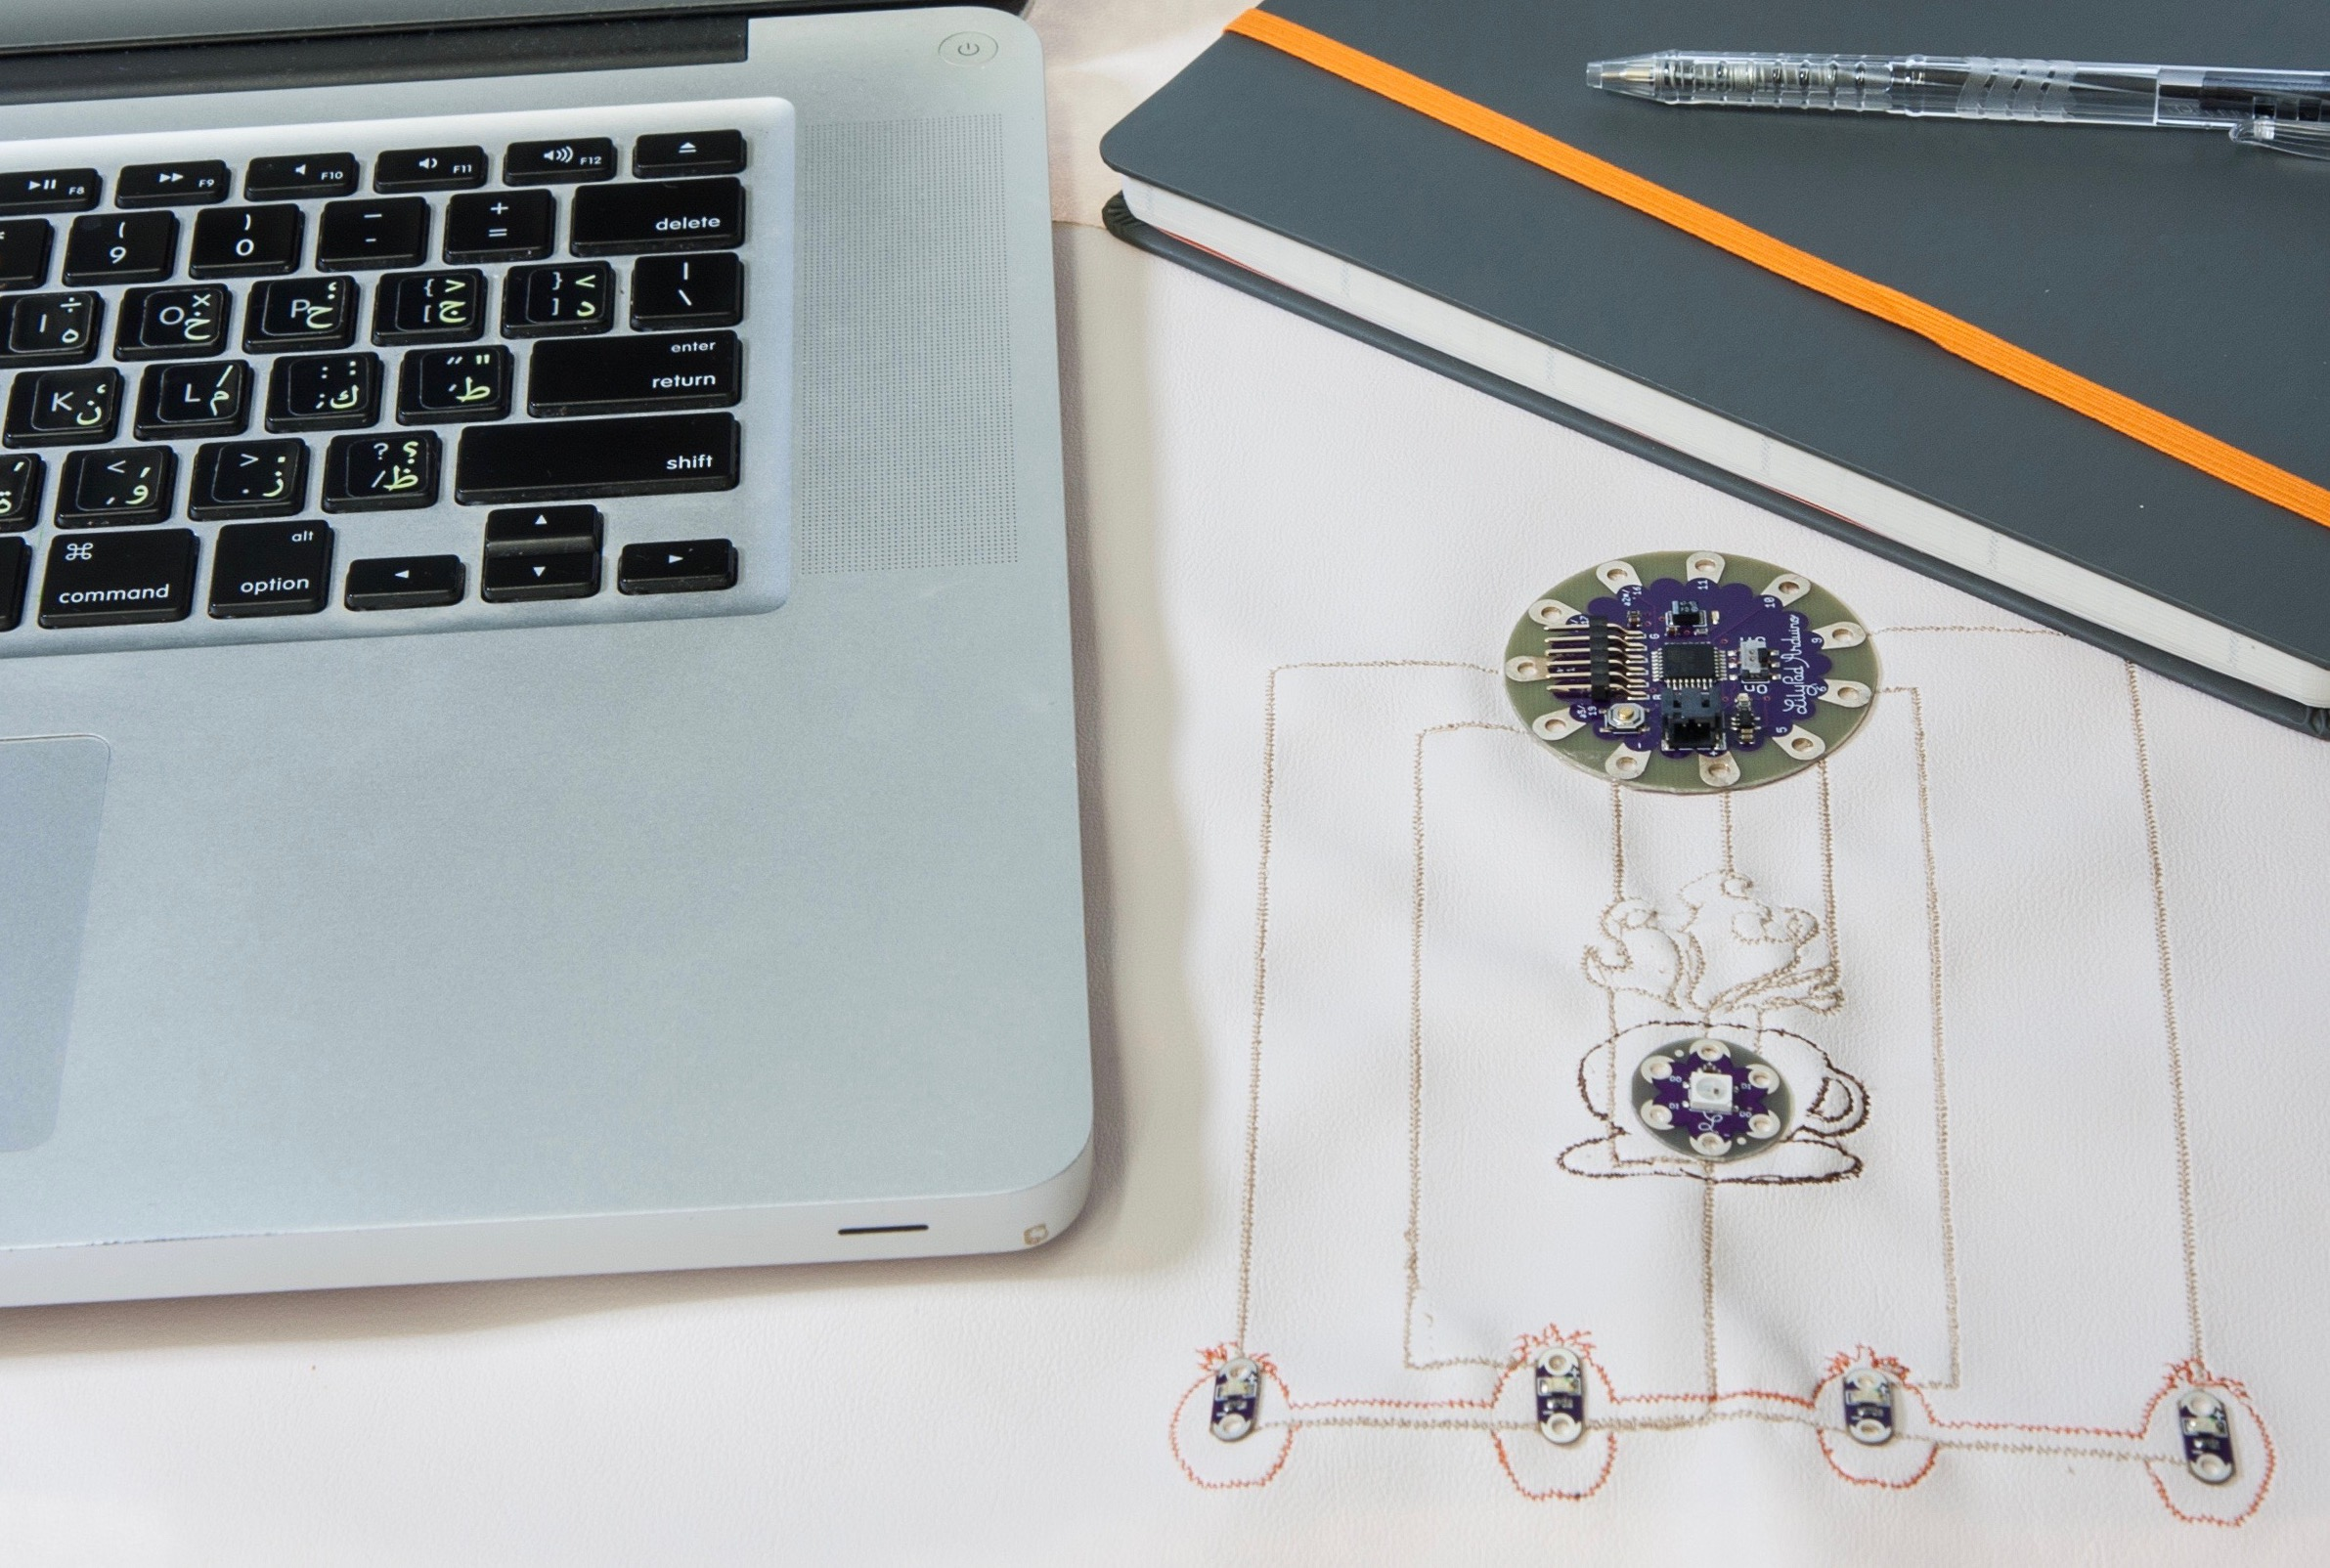
\includegraphics[width=1\columnwidth]{figures/DeskMat}
  \caption{Example 2: The Interactive Desk Mat. Size 160$\times$130 mm, 9,000 stitches, 3 thread changes, 13 minutes stitch duration.}~\label{fig:DeskMat}
  \vspace{-1.5em}
\end{figure}
The second example is an interactive leather desk mat. The artist designed an interface for the ``Pomodoro'' time management technique, using 4 LEDs, a pixel board, and a controller. She plugged the controller into her computer to power it. A timer was programmed to light up an LED every 25 mins to indicate the start of a work interval. Between each work interval, the pixel board flashed to announce a 5 min break. Once all 4 LEDs were lit up, the pixel board lit up to announce a longer break. In her design, the artist used a ruler to draw straight circuit traces for the LEDs. 
%Technical lines seemed appropriate for the context of this application. 
She sketch the traces as part of the art---the steam coming out of the coffee cup was used to connect traces at the center of her artwork. 


\subsection{One-Hour Nap Pillow}
\begin{figure} [h!]
\centering
  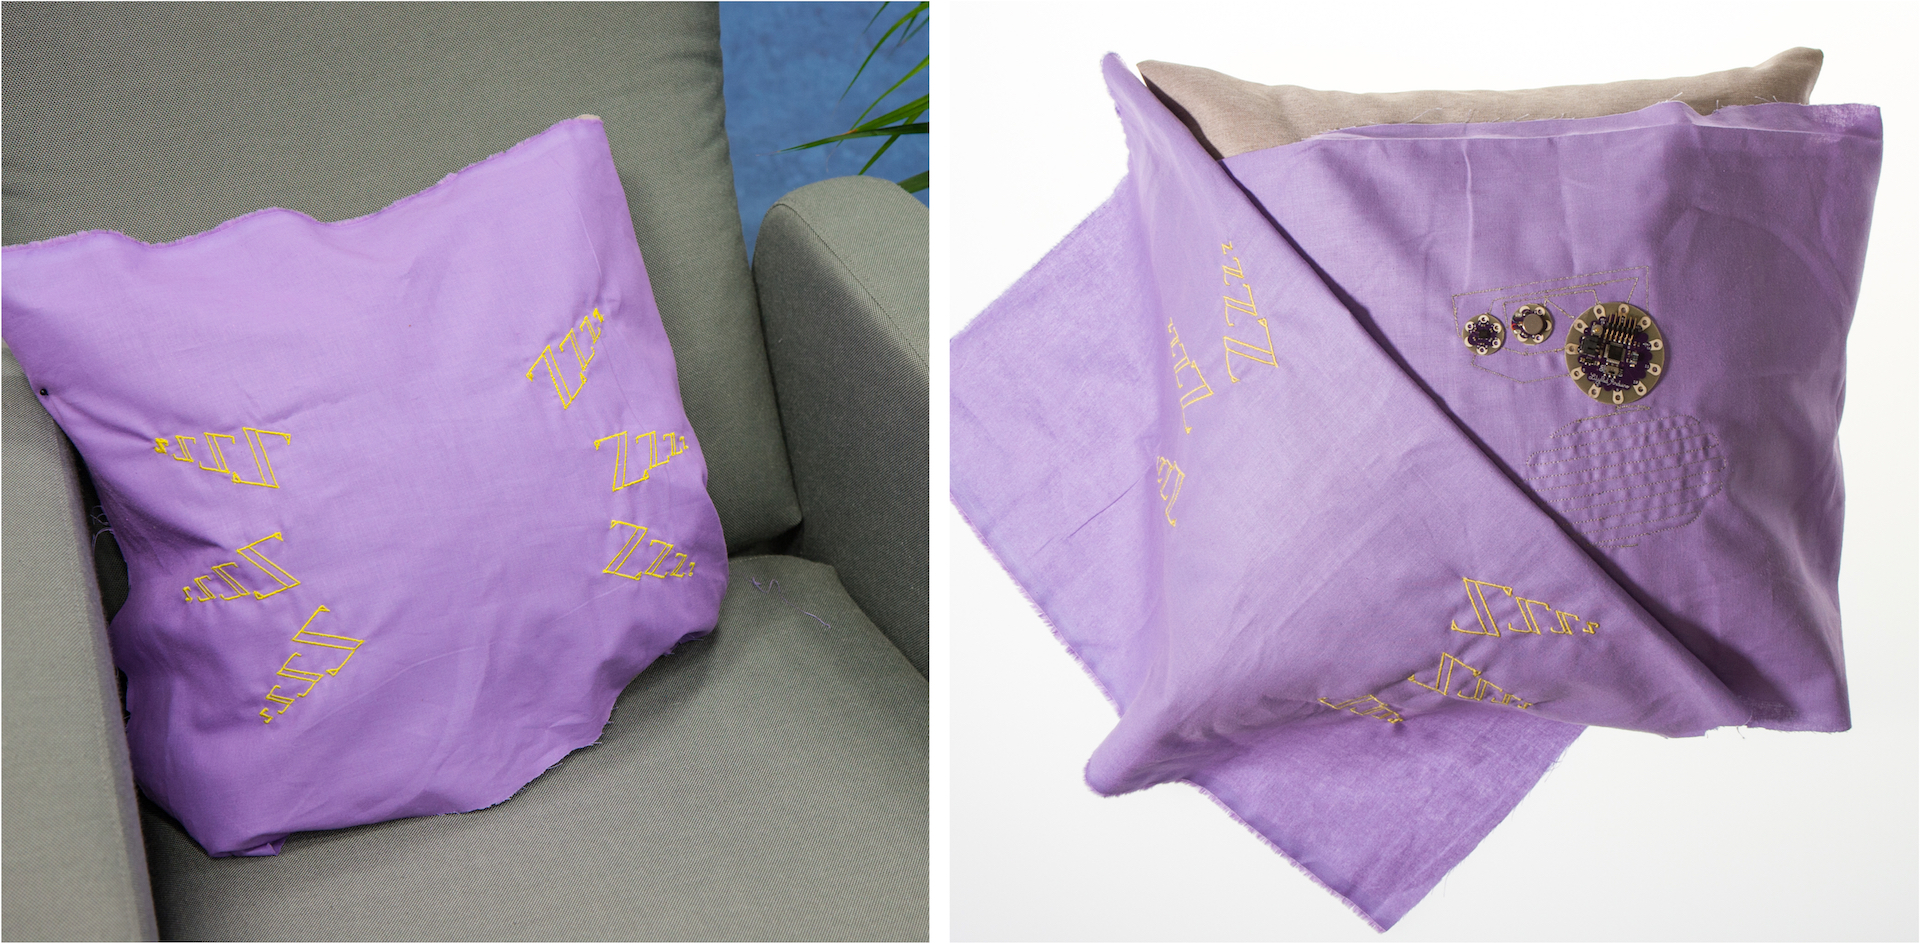
\includegraphics[width=1\columnwidth]{figures/Pillow}
  \caption{Example 3: The One-Hour Nap Pillow. 16,000 stitches, 2 thread changes, 23 minutes stitch duration}~\label{fig:Pillow}
  \vspace{-1.5em}
\end{figure}
The one-hour nap pillow contains a touch sensor that detects when a person first puts their head on the pillow, and awakens him gradually using different vibration patterns after one hour of continuous contact. The user can snooze the pillow by shaking it. An accelerometer signals a 5- or 10-minute snooze based on shaking intensity. The pillow consists of two fabric layers: the lower layer contains the touch sensor and circuit (third concealing strategy), and the top layer is embroidered with a simple artwork. The artist sketched the artwork on one side of the pillow case. She then used the embroidery machine's touch display to mirror and stitch the pattern also onto the other side. 


\subsection{User Feedback and Emerging Design Process}
Overall, the artist was positive about her experience with the Sketch\&Stitch system. She found communicating with the system using marker colors and stickers to be very easy to learn and apply. She felt inspired by the range of methods that Sketch\&Stitch offers to integrate the art and circuit parts of an e-textile. Designing directly on fabric allowed the artist to evaluate her design in real-life. For example, while sketching the Wearable Mandala, the artist wore the t-shirt several times to asses how the design looked or constrained her. She also found that sketching on textures like leather inspired straight lines and right angles, while cotton afforded curved and flowing lines. However, the artist found that not all fabrics afford sketching on them, e.g., towel fabric and fur. Textured fabrics, such as upholstery fabric, required sketching over a single line several times to seal all the gaps caused by the rough surface. Finally, while Sketch\&Stitch reduces the stitching time of an e-textiles, considerable time is still needed to plan and rout the circuit. For example, the artist spent 4 hours on the Wearable Mandala: 30 minutes stitching, 10 minutes attaching the electronics using Z-tape, and the remaining time was split between sketching and circuit routing.

Stickers first


\textit{Scribble on paper and commit on fabric}. The artist always started doodling her initial ideas on paper prior to sketching on fabric. She did not perceive fabric as a medium for scribbling. Even with undo capabilities, she was hesitant to ``waste a good piece of fabric''. 
%She also planed the circuit using Circuit Stickers on paper. 
Once she developed her design idea, she started sketching on fabric. However, she reported that working on fabric still allowed her to visualize the final product better, and sometimes made her make changes to her original design, e.g., strategically repositioning Circuit Stickers on a shirt to convey the design idea.

\textit{Sketch to fit a circuit.} In one of her projects, the artist printed a design inspiration she found online and used it to sketch her circuit. She placed Circuit Stickers on the printed paper and drew traces following design contours. Once she was satisfied with the circuit, she started to sketch her version of the design on fabric with the adaptations. She reported that this technique allowed her to sketch an artwork that fits a circuit instead of fitting a circuit into a design.

\textcolor{red}{
\textit{Integrate or hide.} The artist noted that sometimes she was able to incorporate circuit traces in her design but not circuit boards and components, and sometimes the reverse. Sketch\&Stitch supports both situations using the layered fabric technique to hide parts of the circuit.
}

\section{Limitations and Future work}

Sketch\&Stitch has several important limitations. Since the system depends on a color scheme to process and recognize the user's sketch, users are limited to a range of distinguishable marker colors (their choice of thread colors is only affected if they stitch in iterations.)
In addition, the system can only recognize sketches on fabric of solid colors. Drawings on patterned and dark fabrics are very challenging to capture.  
Drawing on textured fabric can lead to path discontinuities and variations in sketch colors due to change in pressure applied to the marker. For these materials, gestural interaction and projection-based feedback may be beneficial. Finally, the system supports two types of stitches---one for filling and one for lines and outlines. Tool proxies with design constraints \cite{mueller2012interactive} could be used to define other stitch types.


As Sketch\&Stitch automates the conversion of freehand sketches to embroidery patterns, jump stitches are very frequent and require trimming to avoid short circuits. High-end embroidery machines offer automatic trimming with a penalty of increased embroidery time. For fewer jump stitches, we could reorder the embroidery sequence of individual stitch objects algorithmically.

Finally, the current version of Sketch\&Stitch does not offer the autorouting and design rule checks for fabric circuits known from PCB layout tools. While users can test their circuit early and frequently in the design process, we believe that embroidery should offer an opportunity for circuit design and validation. Eichinger et al.\ \cite{eichinger2007using} presented early work on using PCB layout software (Eagle) to create embroidered fabric circuits. 
%However, they targeted people who are familiar with PCB layout software.
In future work, we would like to examine how to auto-route circuit traces based on the outlines of the artwork, inspired by \cite{savage2014series}.

One way to improve the accuracy of a capacitive touch sensor is to maintain a constant base capacitance, used as a reference for each measurement. Base capacitance is affected by environmental effects such as temperature and humidity. Texas Instruments for PCB-based capacitive touch sensing \footnote{www.ti.com/lit/an/slaa363a/slaa363a.pdf} recommends two methods for handling this: (1) shielding the sensor with a bottom layer 50\%--75\% hatched ground pour to isolate it from potential
interference, e.g., from contact with the skin; and (2) constantly monitoring and tracking variation in base capacitance using, e.g., Derivative Integration Algorithm \footnote{http://www.ti.com/lit/an/snoa939/snoa939.pdf}, for correct comparison to
touch events.




%Our capture system cannot distinguish between overlapping lines in a single connection and between two connection.

%The camera capture setup should be well lit to avoid noise from shadows and inconsistent light. 

%In this paper we mainly focused on LilyPad electronics kit. Sketch\&Stitch ca support any off-the-shelf electronics, including DIP and SMD packages, as long as they have a 2.5 mm pitch between leads.
%%trade off between reliable contact surface and smaller contact points.

%The next step for conductive embroidery is to examine using the conductive bobbin thread together with conductive top thread to create multi-layer electrical devices.  

%Ultimately an embroidery machine can be adapted to work like a pick and place machine---placing and stitching electronic components on fabric based on design file. 


\section{Conclusion}
This paper described Sketch\&Stitch, a proof-of-concept system for fabricating e-textiles. The system combines physical sketching with a computerized embroidery machine offering users the benefits of direct making and the power of digital tools. The system is targeted at artists, designers, and makers especially during the early stages of e-textile design. We demonstrated the advantages of our design pipeline.


Particular advantages of embroidery machines for e-textile fabrication are that (a) they produce very accurate and consistent stitches over a relatively large surface, (b) their speed, (c) embroidery patterns of circuit elements such as sensors, passive components, antennas, etc., can be pre-programmed, modified, shared, and reused, always providing consistent results, (d) they can be programmed to automatically shield circuit traces, (e) embroidery is an additive manufacturing process that can be use on tailored and finished textiles, 
%reduces the waist created from e-textile fabrication, 
and finally (f) they are accessible to end users.


%more agency and control over the final outcome \cite{}
% BALANCE COLUMNS
\balance{}

% REFERENCES FORMAT
% References must be the same font size as other body text.
\bibliographystyle{SIGCHI-Reference-Format}
\bibliography{main}

\end{document}
%%% Local Variables:
%%% mode: latex
%%% TeX-master: t
%%% End:
